\section{Histograms~\label{sec:sodb9_hist}} 
This section exhibits histograms on the EMPv5 data obtained when 
the task length of INC increases from 1 second to 2048 seconds. 
The detailed description of the base data is from Table~\ref{tab:exp_notes}.

\subsection{ET}

\begin{figure}[hp!]
	\centering
	\subfigure[ET frequency on INC1]{
		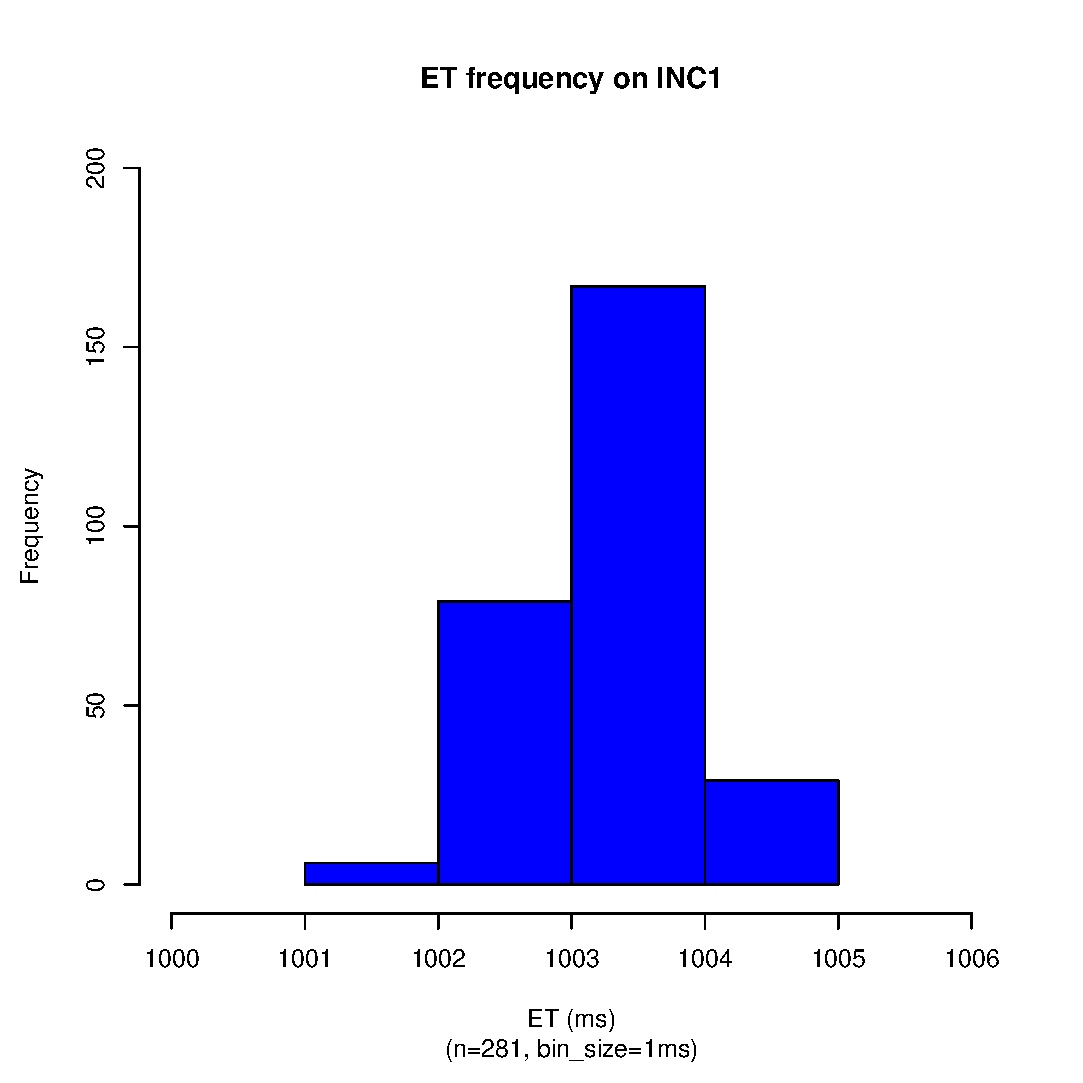
\includegraphics[scale=0.43]{sodb9/1_sec_et_hist_v5.eps}
		\label{fig:inc1_et_hist_v5}
	}
	\subfigure[ET frequency on INC2]{
		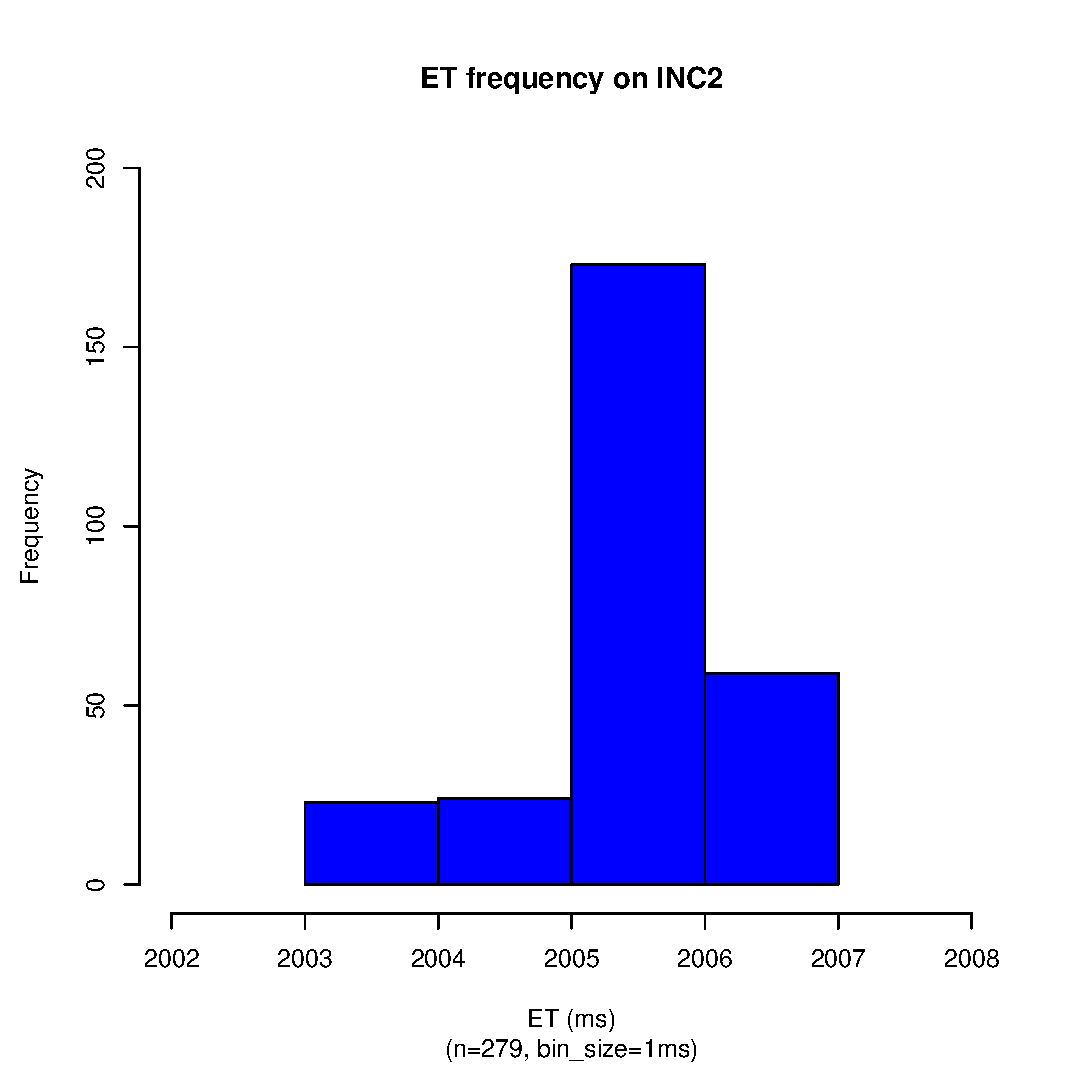
\includegraphics[scale=0.43]{sodb9/2_sec_et_hist_v5.eps}
		\label{fig:inc2_et_hist_v5}
	}
	\subfigure[ET frequency on INC4]{
		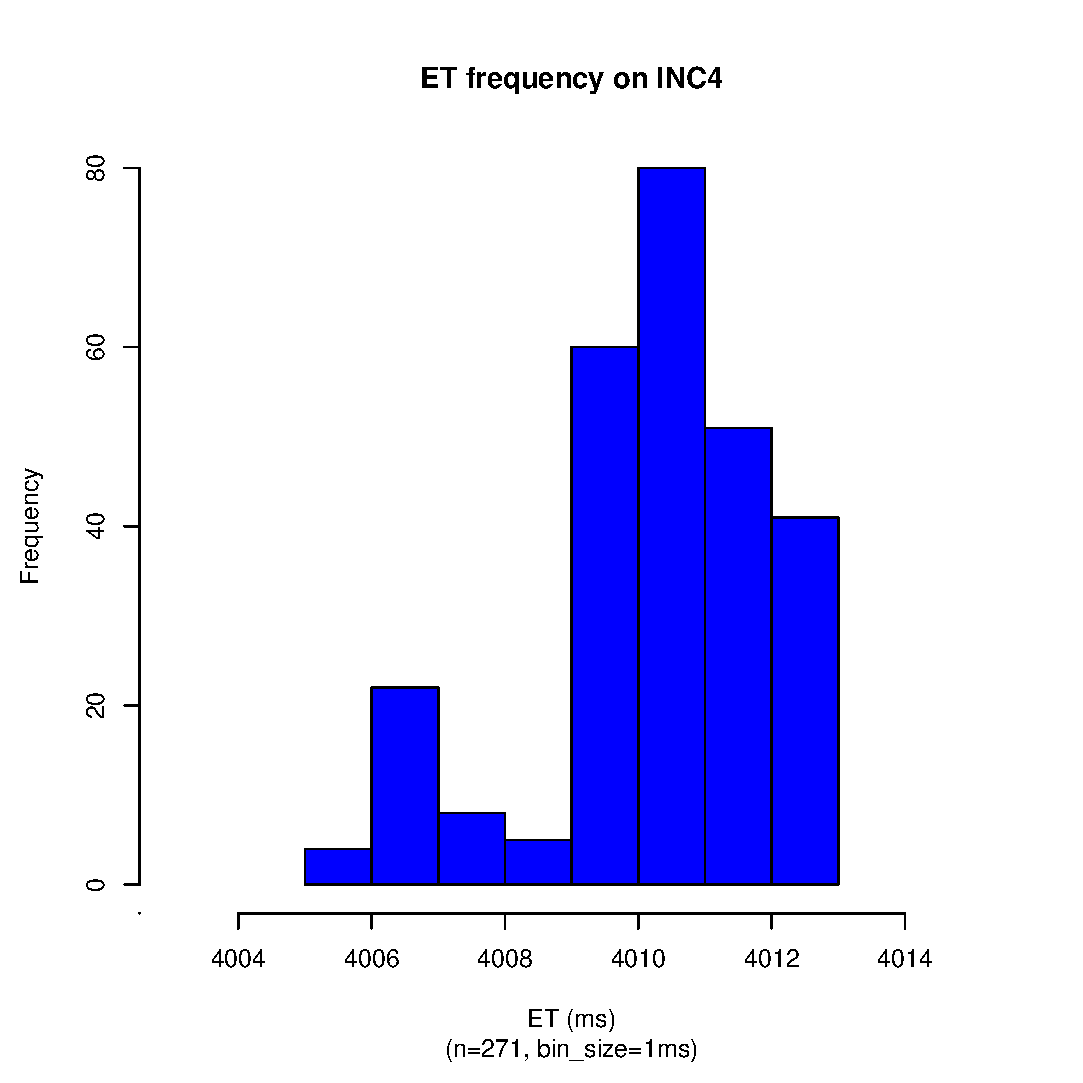
\includegraphics[scale=0.43]{sodb9/4_sec_et_hist_v5.eps}
		\label{fig:inc4_et_hist_v5}
	}
	\subfigure[ET frequency on INC8]{
		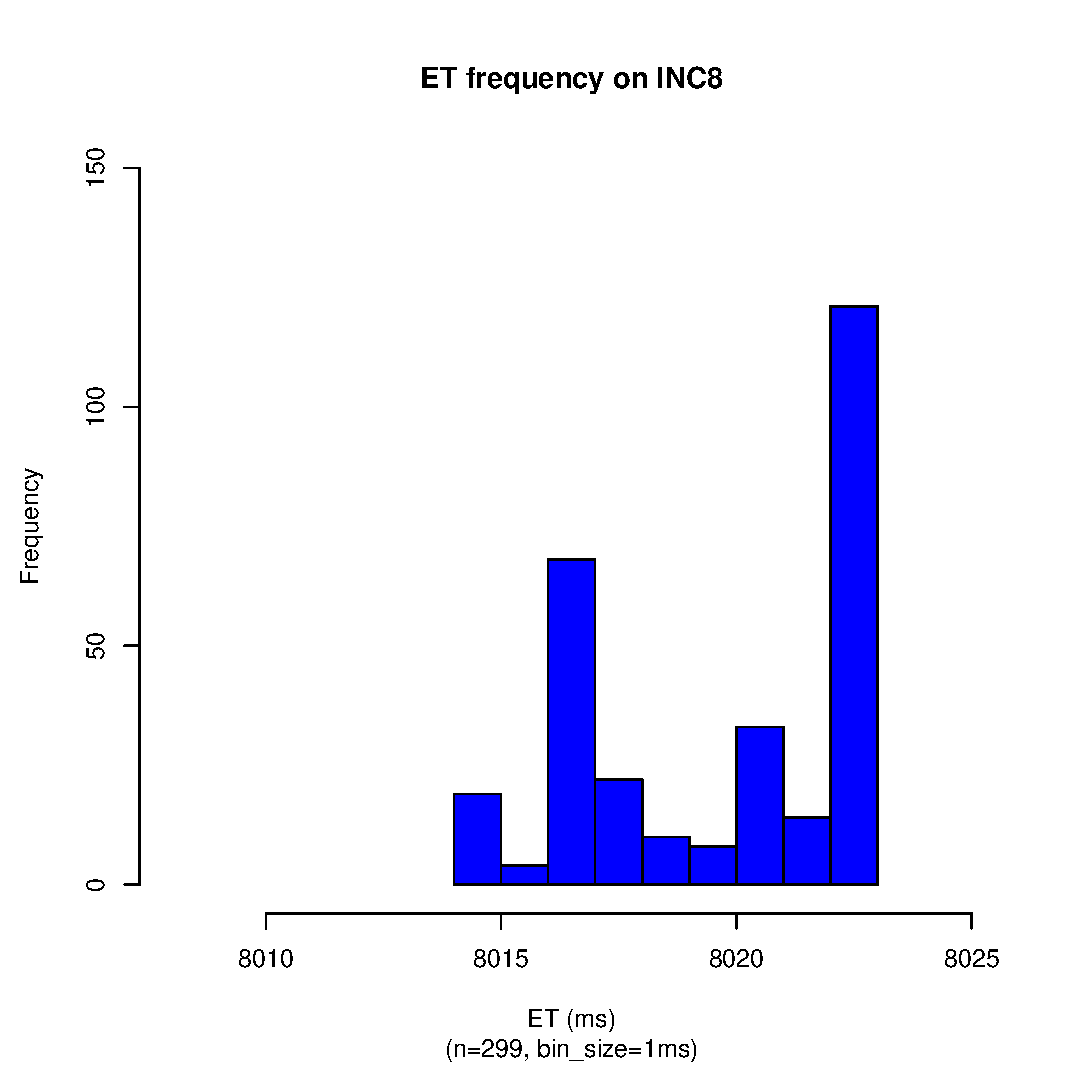
\includegraphics[scale=0.43]{sodb9/8_sec_et_hist_v5.eps}
		\label{fig:inc8_et_hist_v5}
	}
	\caption{ET Histograms of INC1 ... INC8~\label{fig:s9_et_hist1}}
\end{figure}

\begin{figure}[hp!]
	\centering
	\subfigure[ET frequency on INC16]{
		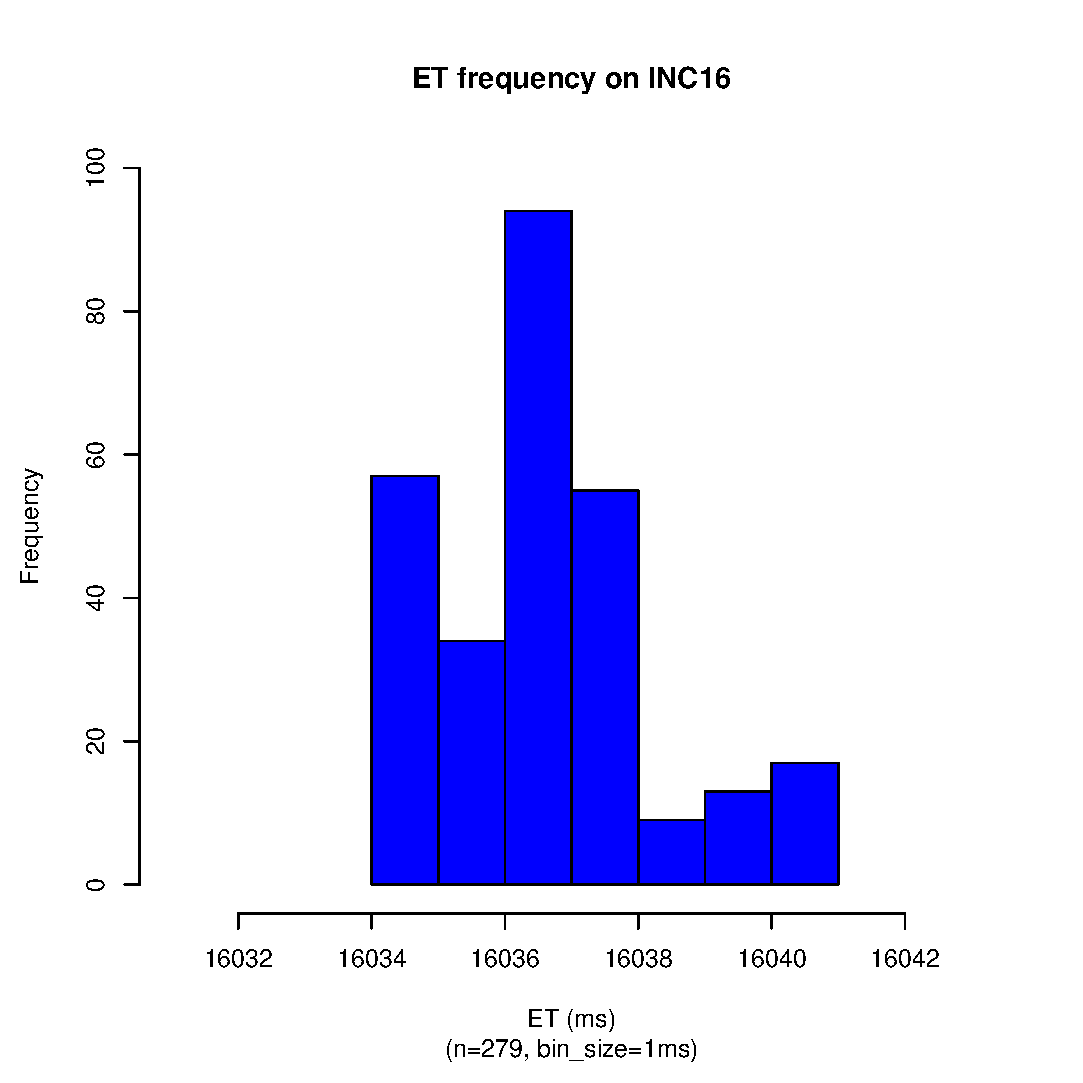
\includegraphics[scale=0.43]{sodb9/16_sec_et_hist_v5.eps}
		\label{fig:inc16_et_hist_v5}
	}
	\subfigure[ET frequency on INC32]{
		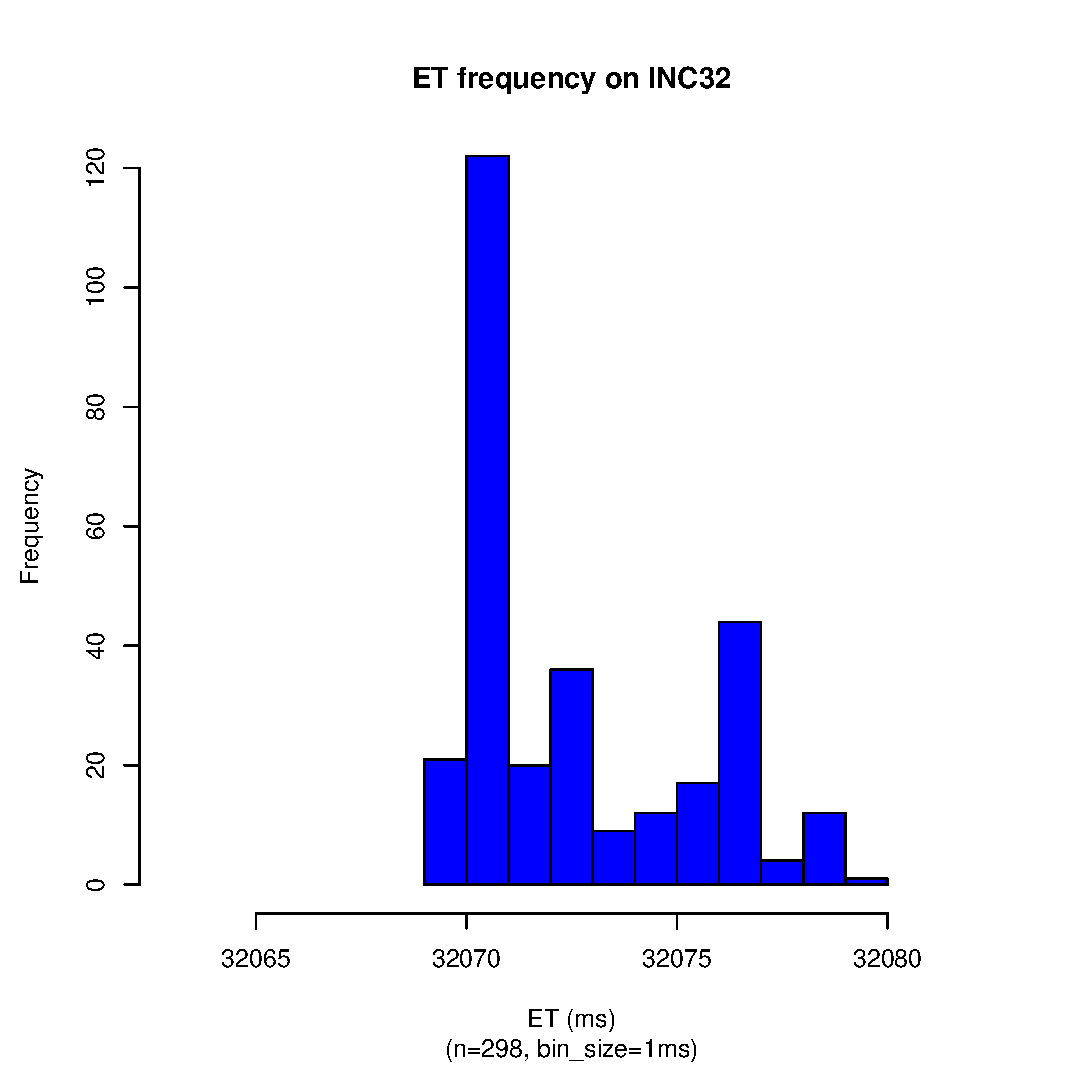
\includegraphics[scale=0.43]{sodb9/32_sec_et_hist_v5.eps}
		\label{fig:inc32_et_hist_v5}
	}
	\subfigure[ET frequency on INC64]{
		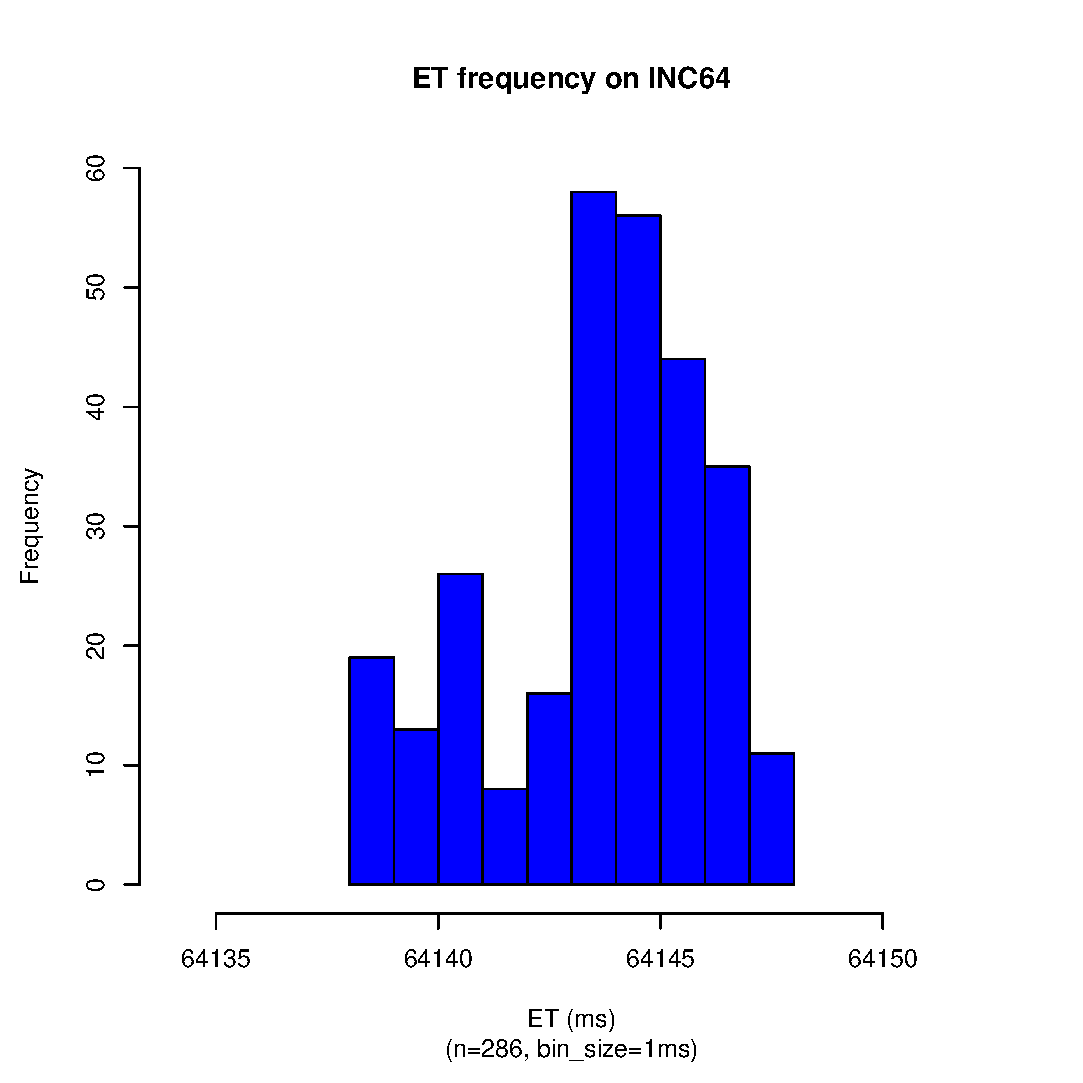
\includegraphics[scale=0.43]{sodb9/64_sec_et_hist_v5.eps}
		\label{fig:inc64_et_hist_v5}
	}
	\caption{ET Histograms of INC16 ... INC64~\label{fig:s9_et_hist2}}
\end{figure}

\begin{figure}[hp!]
	\centering
	\subfigure[ET frequency on INC128]{
		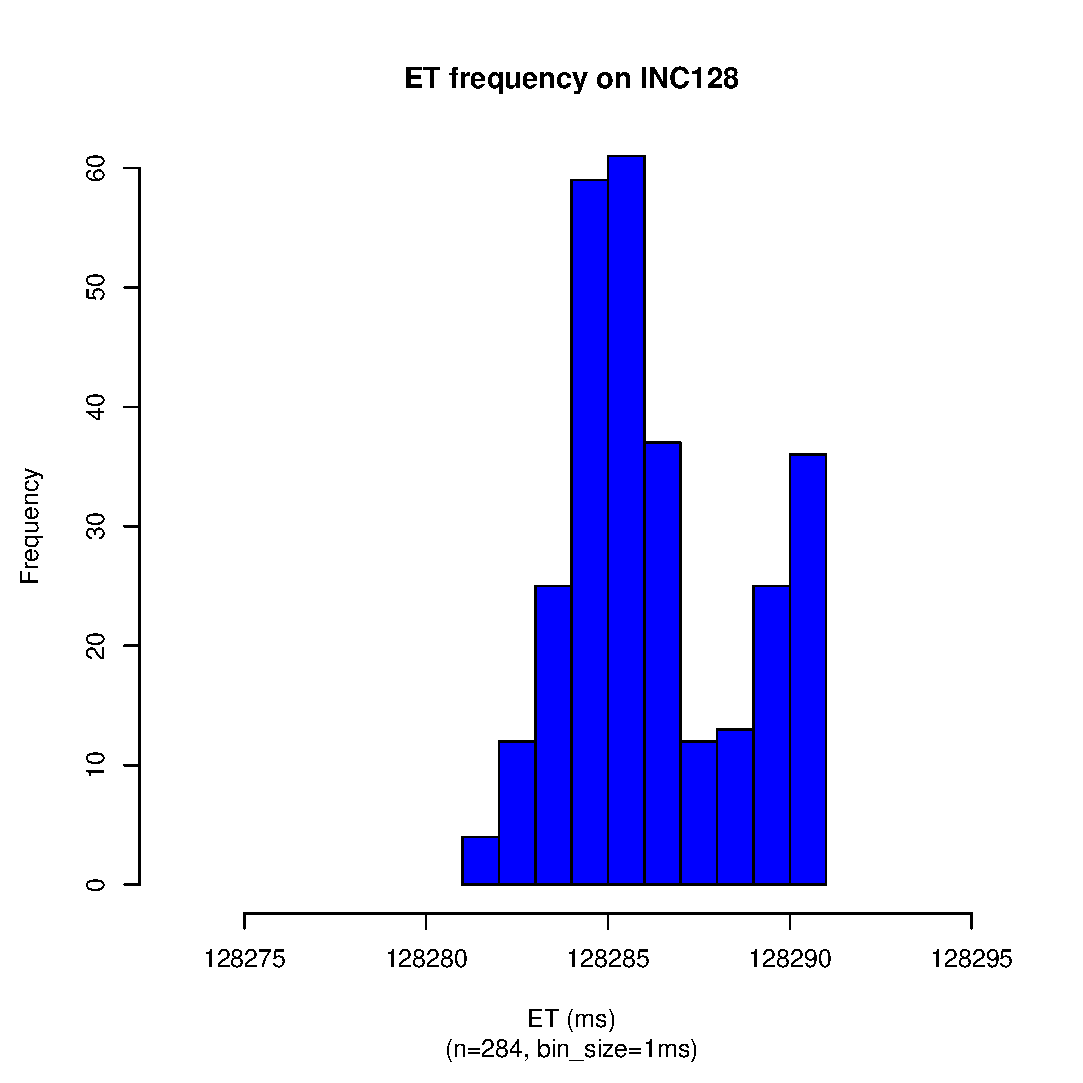
\includegraphics[scale=0.43]{sodb9/128_sec_et_hist_v5.eps}
		\label{fig:inc128_et_hist_v5}
	}
	\subfigure[ET frequency on INC256]{
		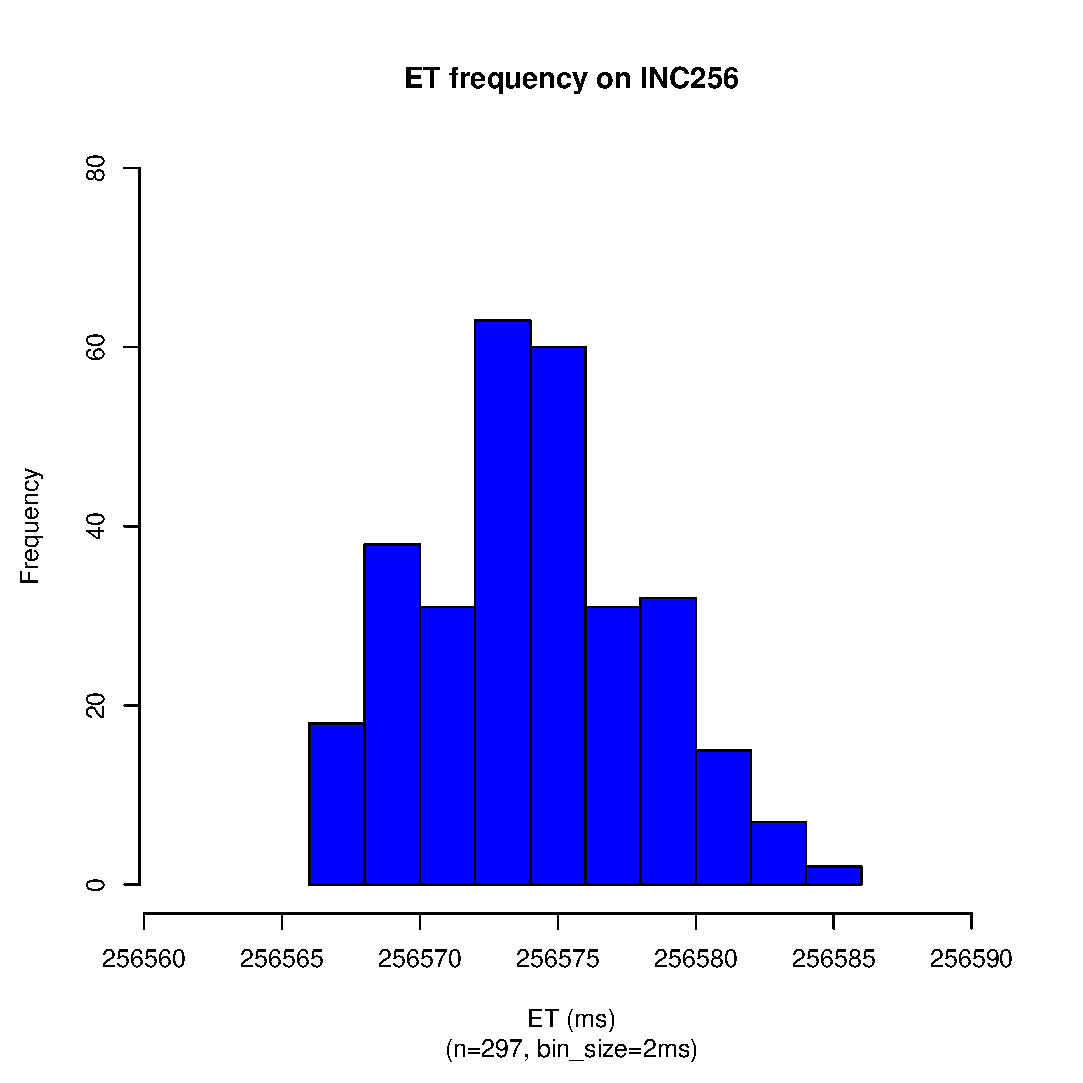
\includegraphics[scale=0.43]{sodb9/256_sec_et_hist_v5.eps}
		\label{fig:inc256_et_hist_v5}
	}
	\subfigure[ET frequency on INC512]{
		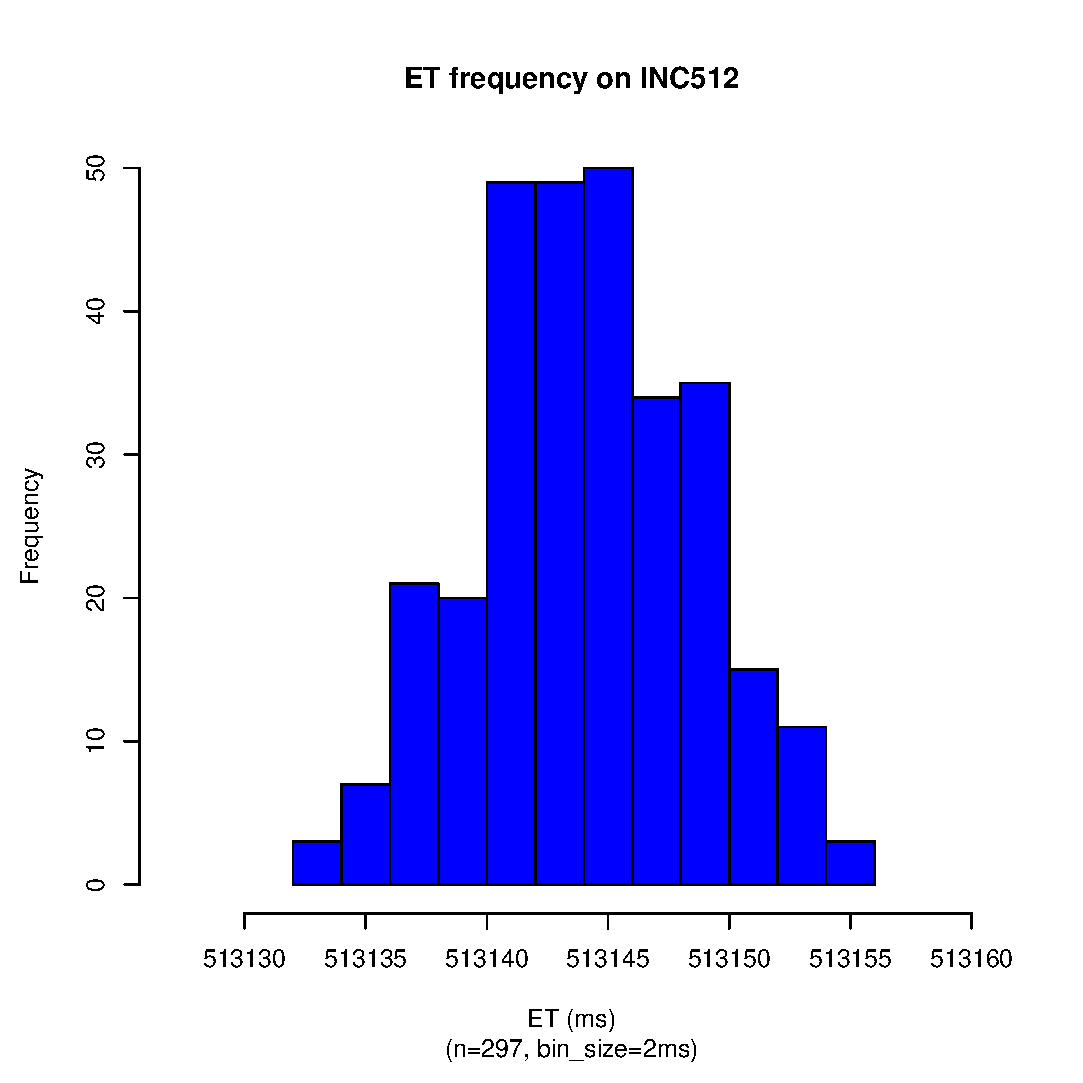
\includegraphics[scale=0.43]{sodb9/512_sec_et_hist_v5.eps}
		\label{fig:inc512_et_hist_v5}
	}
	\subfigure[ET frequency on INC1024]{
		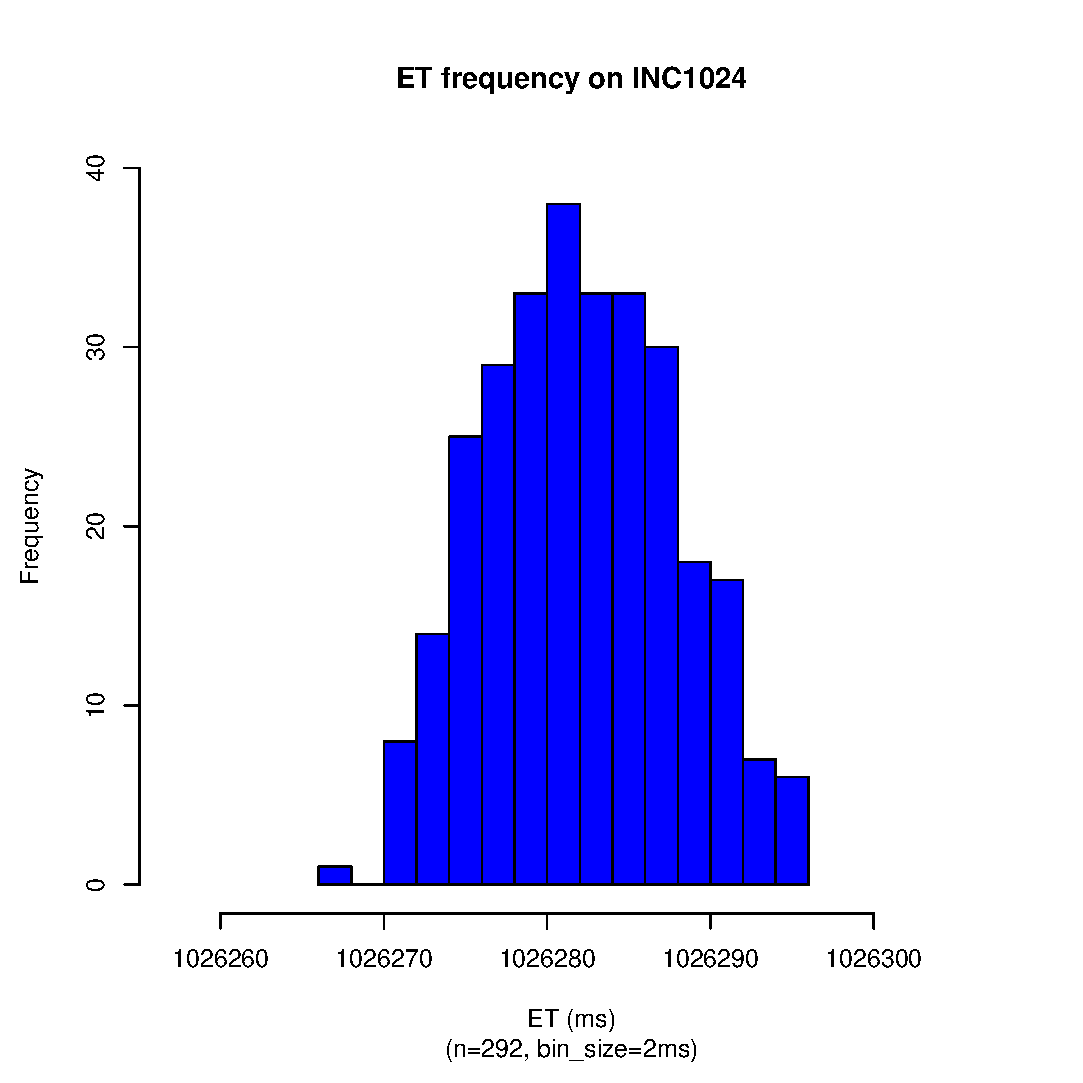
\includegraphics[scale=0.43]{sodb9/1024_sec_et_hist_v5.eps}
		\label{fig:inc1024_et_hist_v5}
	}
	\caption{ET Histograms of INC128 ... INC1024~\label{fig:s9_et_hist3}}
\end{figure}

\pagebreak

\begin{figure}[hp!]
	\centering
	\subfigure[ET frequency on INC2048]{
		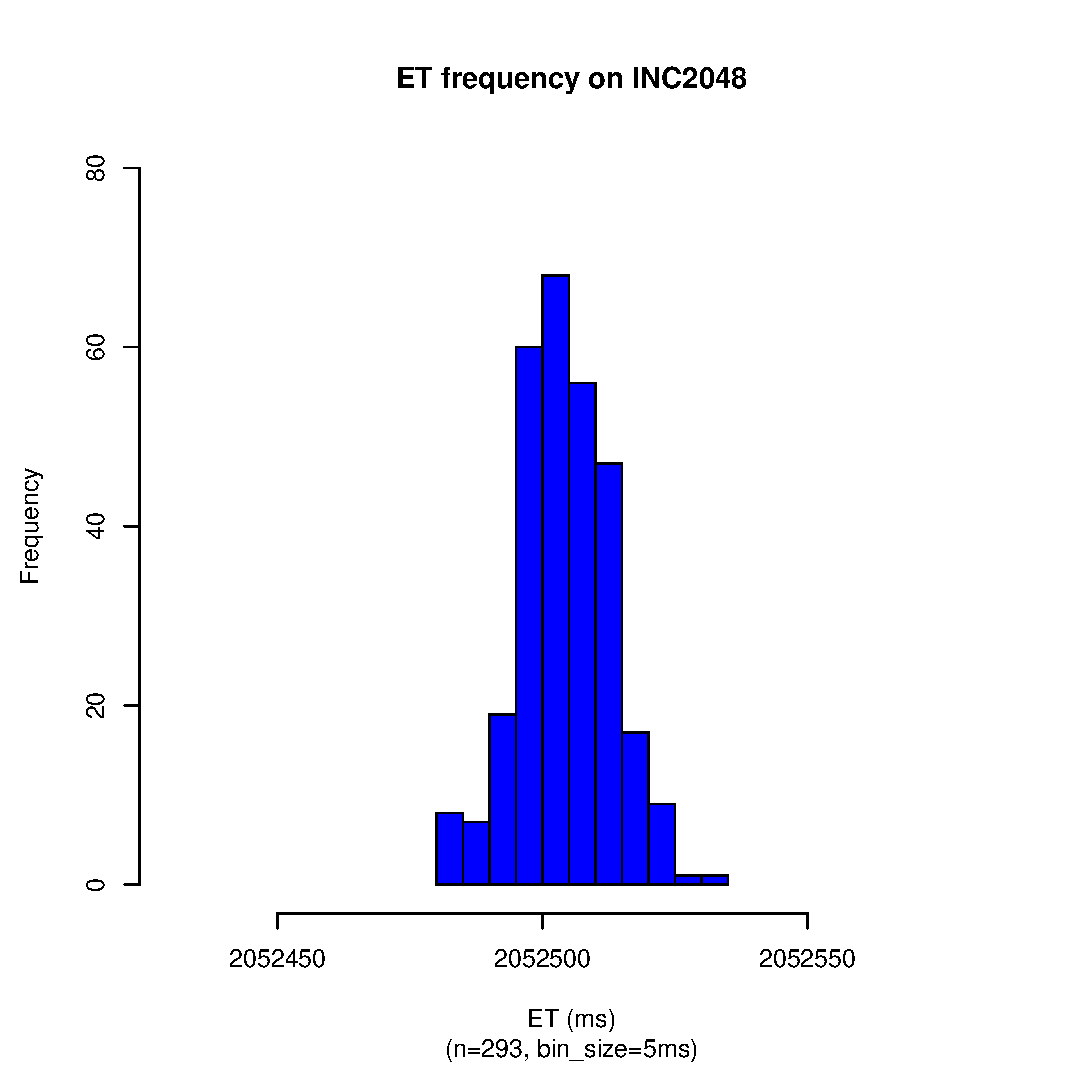
\includegraphics[scale=0.43]{sodb10/2048_sec_et_hist_v5.eps}
		\label{fig:inc2048_et_hist_v5}
	}
	\subfigure[ET frequency on INC4096]{
		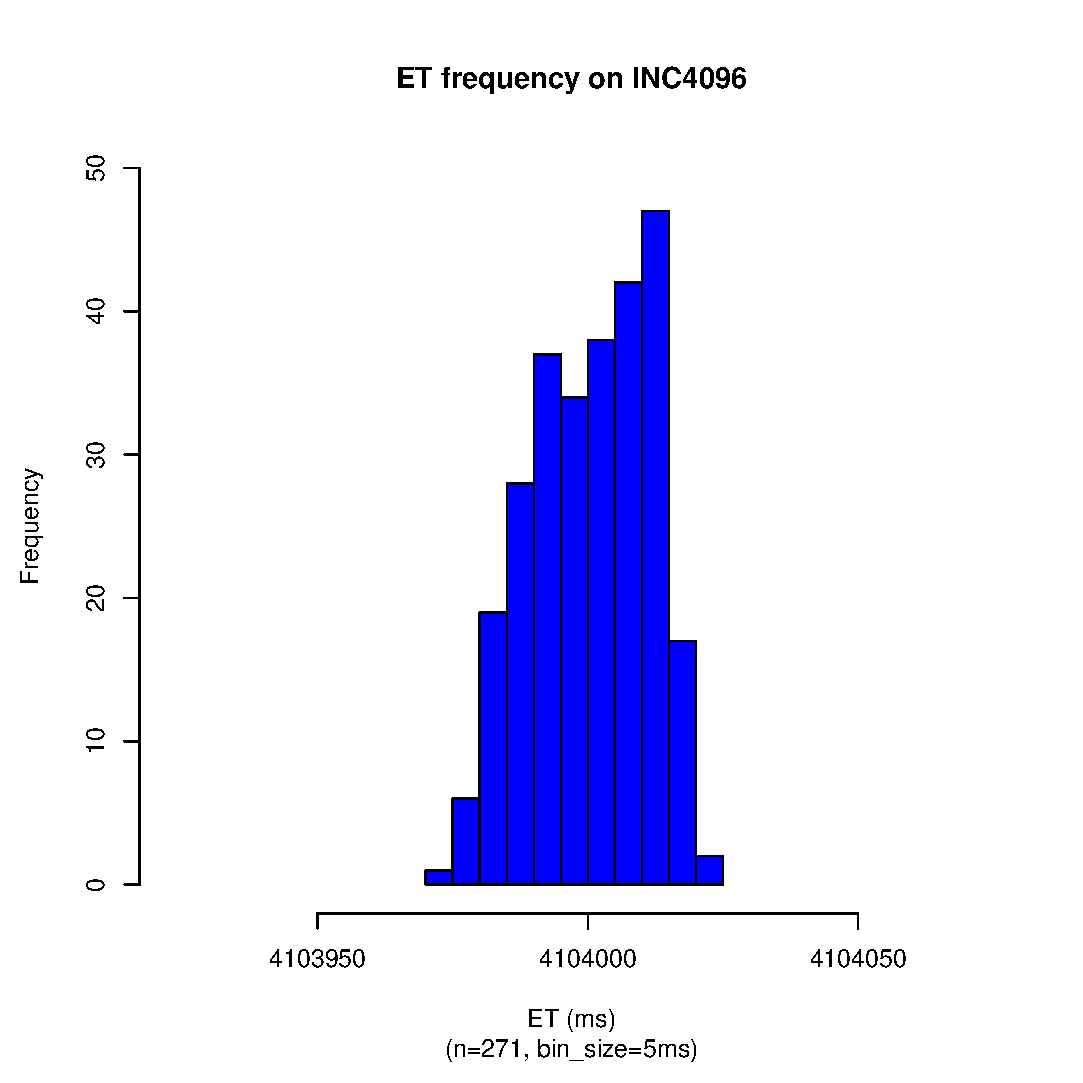
\includegraphics[scale=0.43]{sodb12/4096_sec_et_hist_v5.eps}
		\label{fig:inc4096_et_hist_v5}
	}
	\subfigure[ET frequency on INC8192]{
		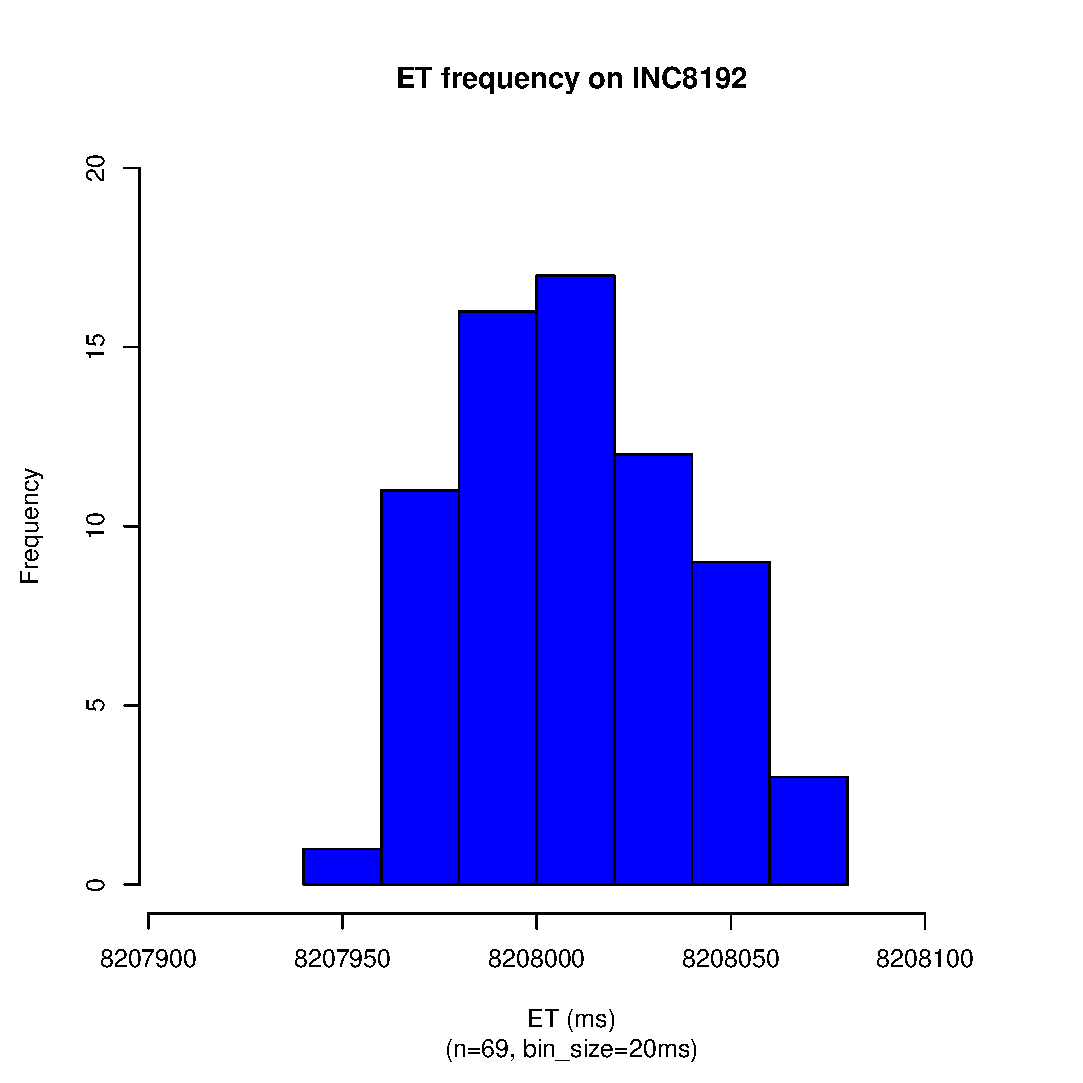
\includegraphics[scale=0.43]{sodb12/8192_sec_et_hist2_v5.eps}
		\label{fig:inc8192_et_hist_v5}
	}
	\subfigure[ET frequency on INC16384]{
		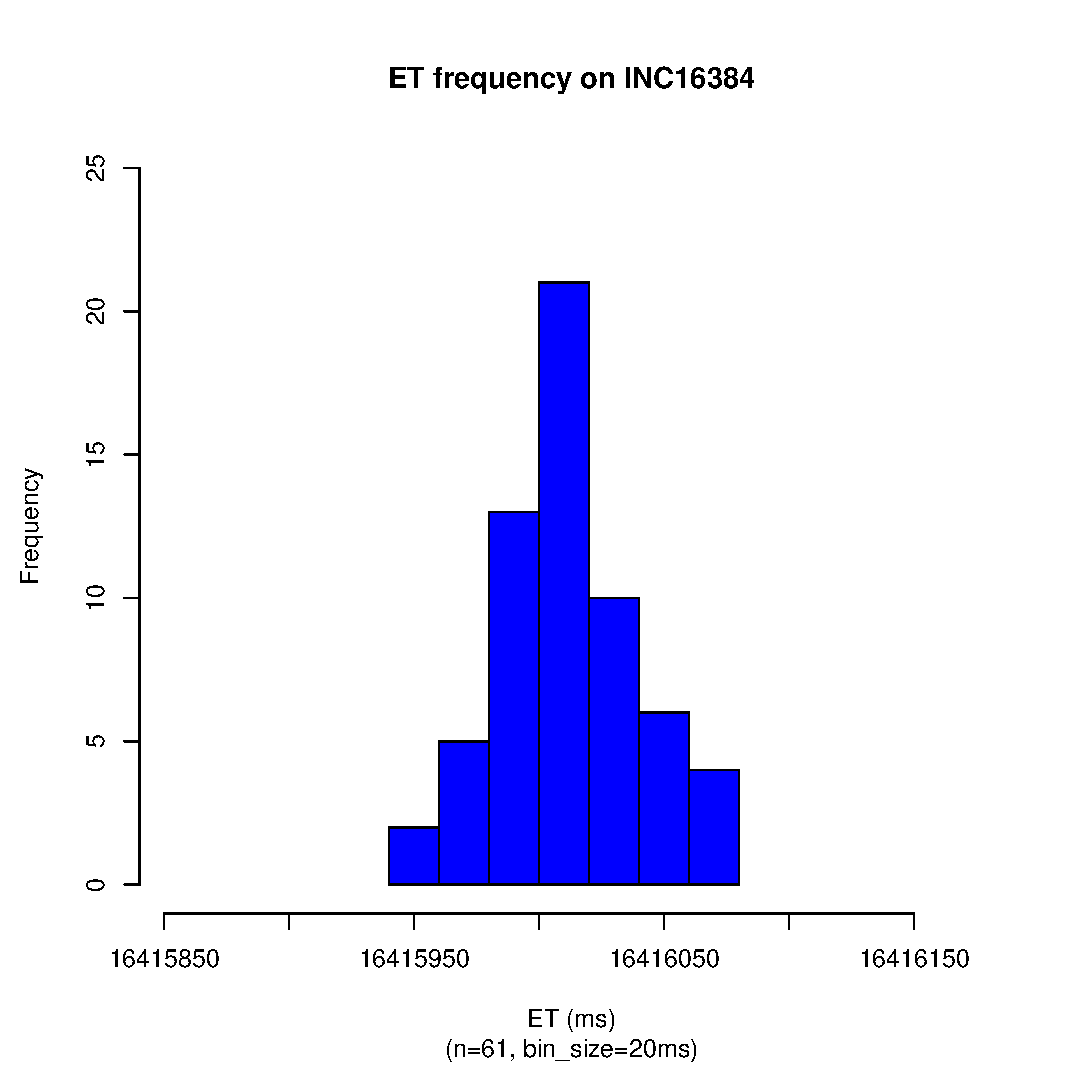
\includegraphics[scale=0.43]{sodb12/16384_sec_et_hist2_v5.eps}
		\label{fig:inc16384_et_hist_v5}
	}
	\caption{ET Histograms of INC2048 ... INC16384~\label{fig:s9_et_hist4}}
\end{figure}

%\pagebreak
%
%\begin{figure}[hp!]
%	\centering
%	\subfigure[ET frequency on INC8192]{
%		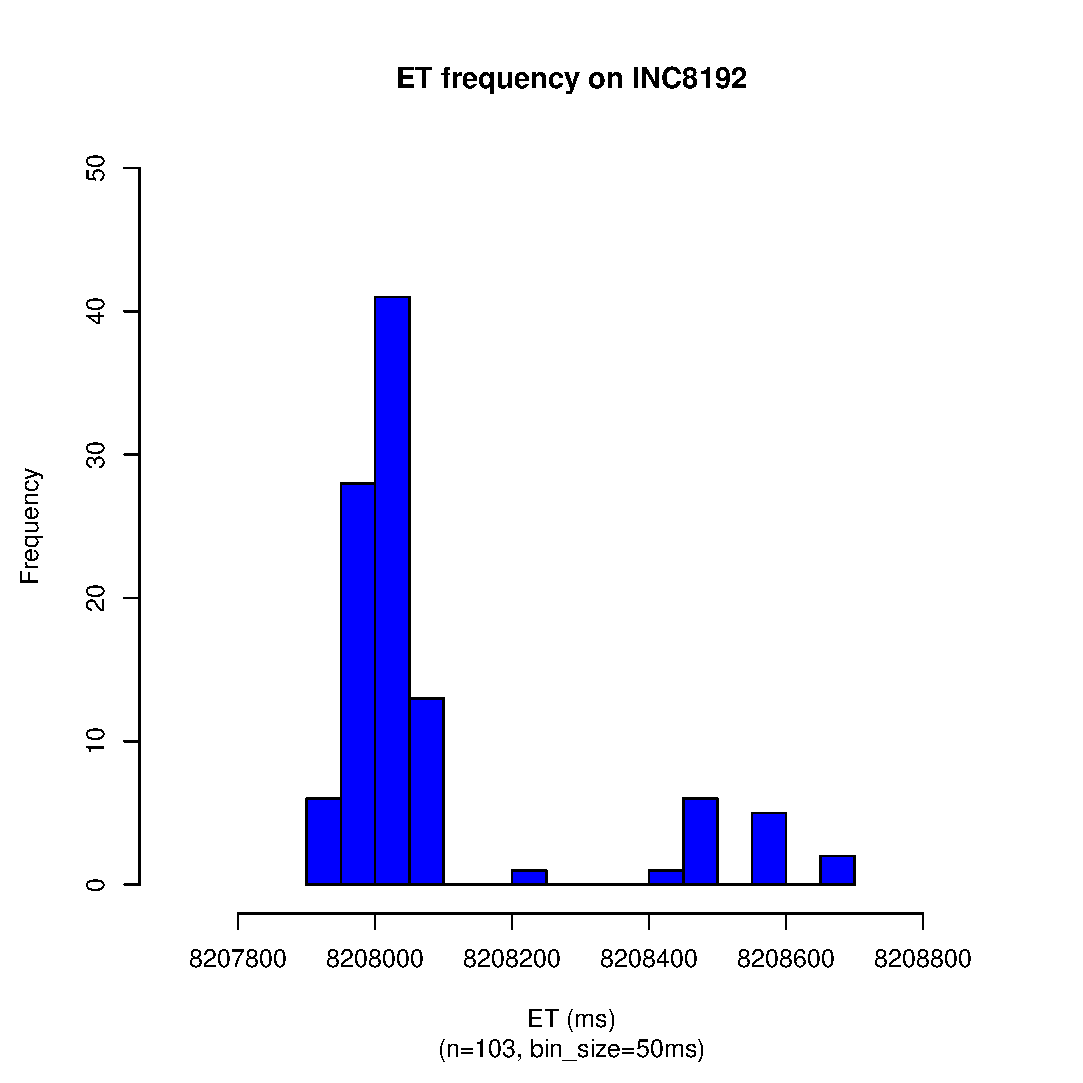
\includegraphics[scale=0.43]{sodb12/8192_sec_et_hist_v5.eps}
%		\label{fig:inc8192_et_hist_all_v5}
%	}
%	\subfigure[ET frequency on INC16384]{
%		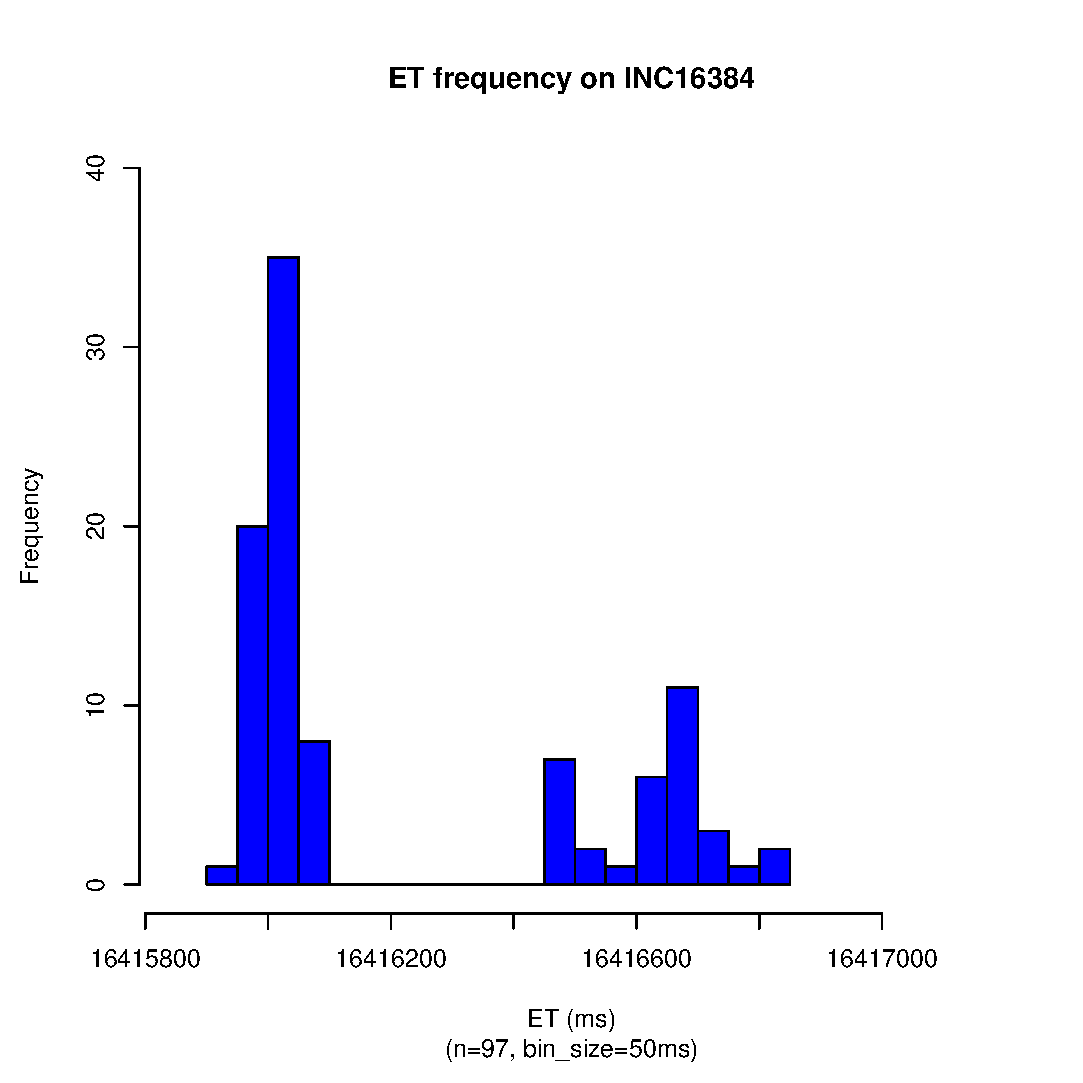
\includegraphics[scale=0.43]{sodb12/16384_sec_et_hist_v5.eps}
%		\label{fig:inc16384_et_hist_all_v5}
%	}
%	\caption{ET Histograms of INC8192... INC16384 [combined with 2015's run]~\label{fig:s9_et_hist5}}
%\end{figure}

\newpage

\subsection{PT}

\begin{figure}[hp!]
	\centering
	\subfigure[PT frequency on INC1]{
		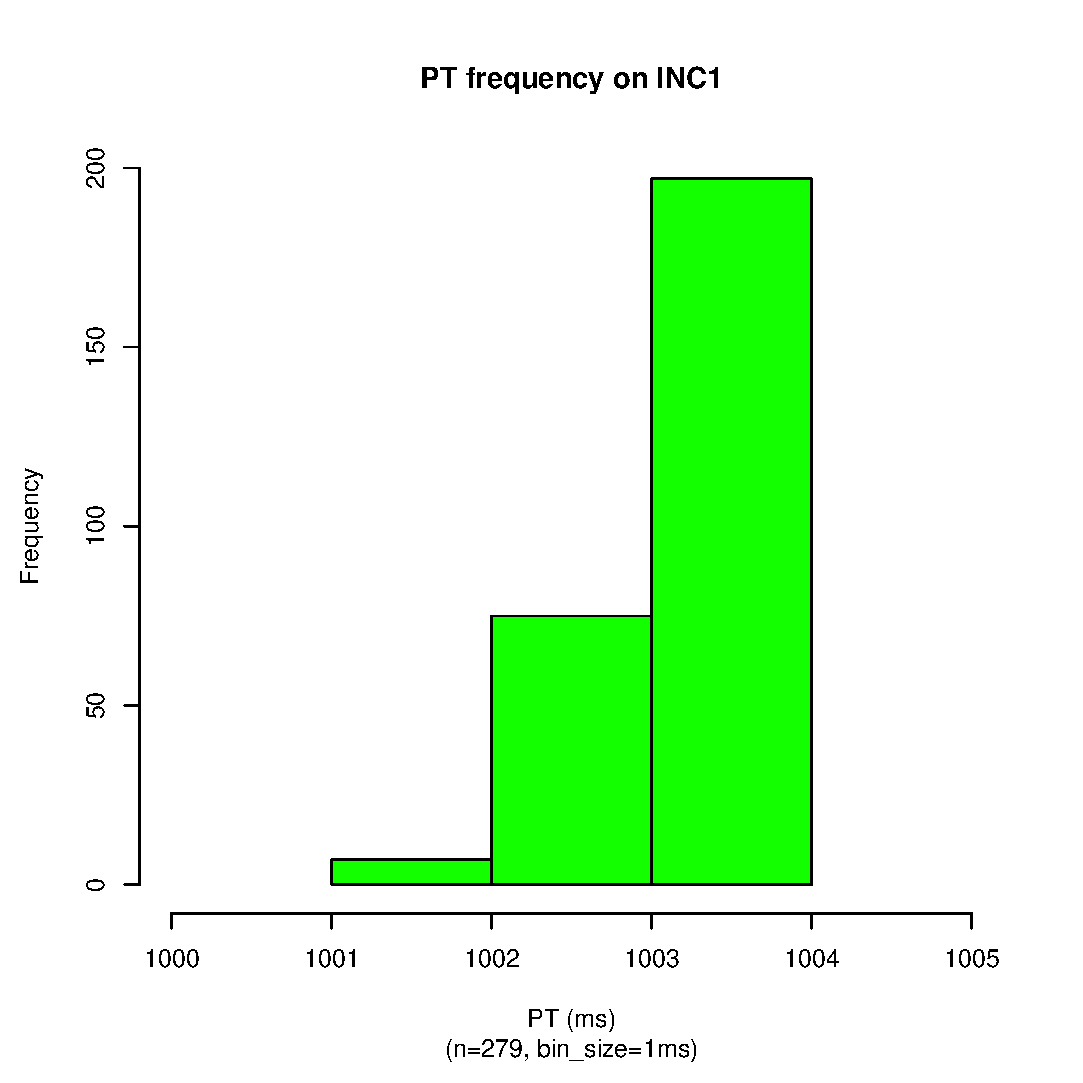
\includegraphics[scale=0.43]{sodb9/1_sec_pt_hist_v5.eps}
		\label{fig:inc1_hist_v5}
	}
	\subfigure[PT frequency on INC2]{
		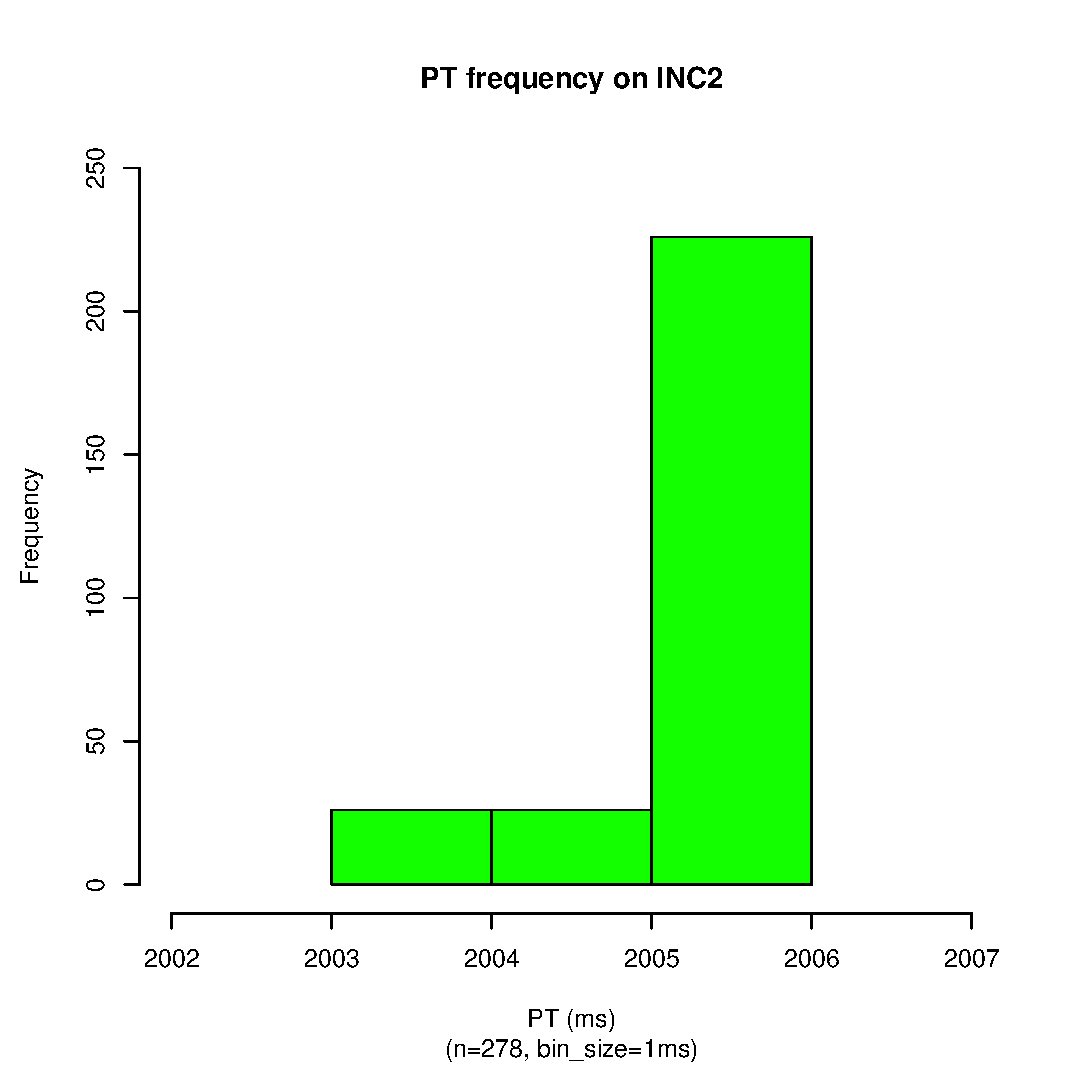
\includegraphics[scale=0.43]{sodb9/2_sec_pt_hist_v5.eps}
		\label{fig:inc2_hist_v5}
	}
	\subfigure[PT frequency on INC4]{
		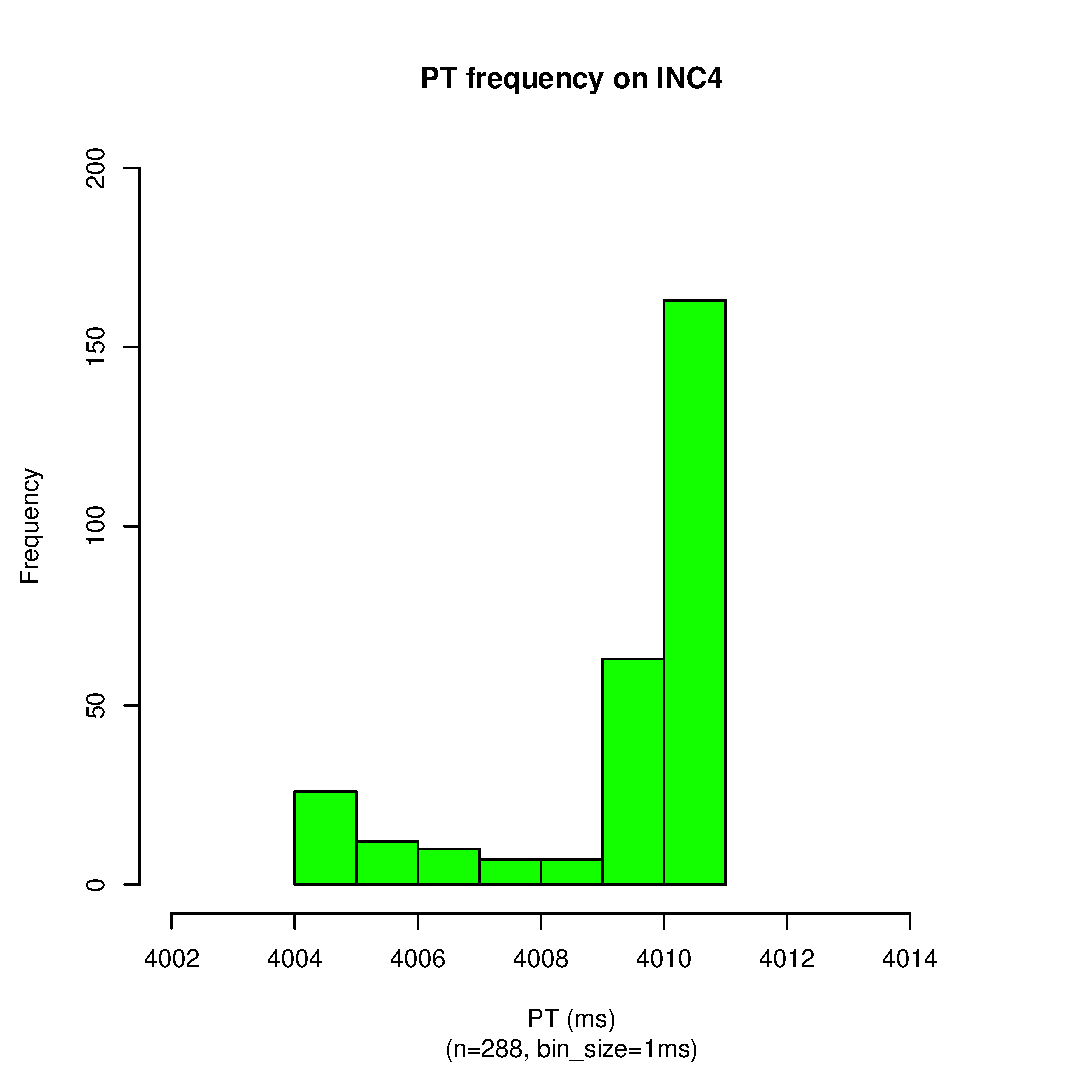
\includegraphics[scale=0.43]{sodb9/4_sec_pt_hist_v5.eps}
		\label{fig:inc4_hist_v5}
	}
	\subfigure[PT frequency on INC8]{
		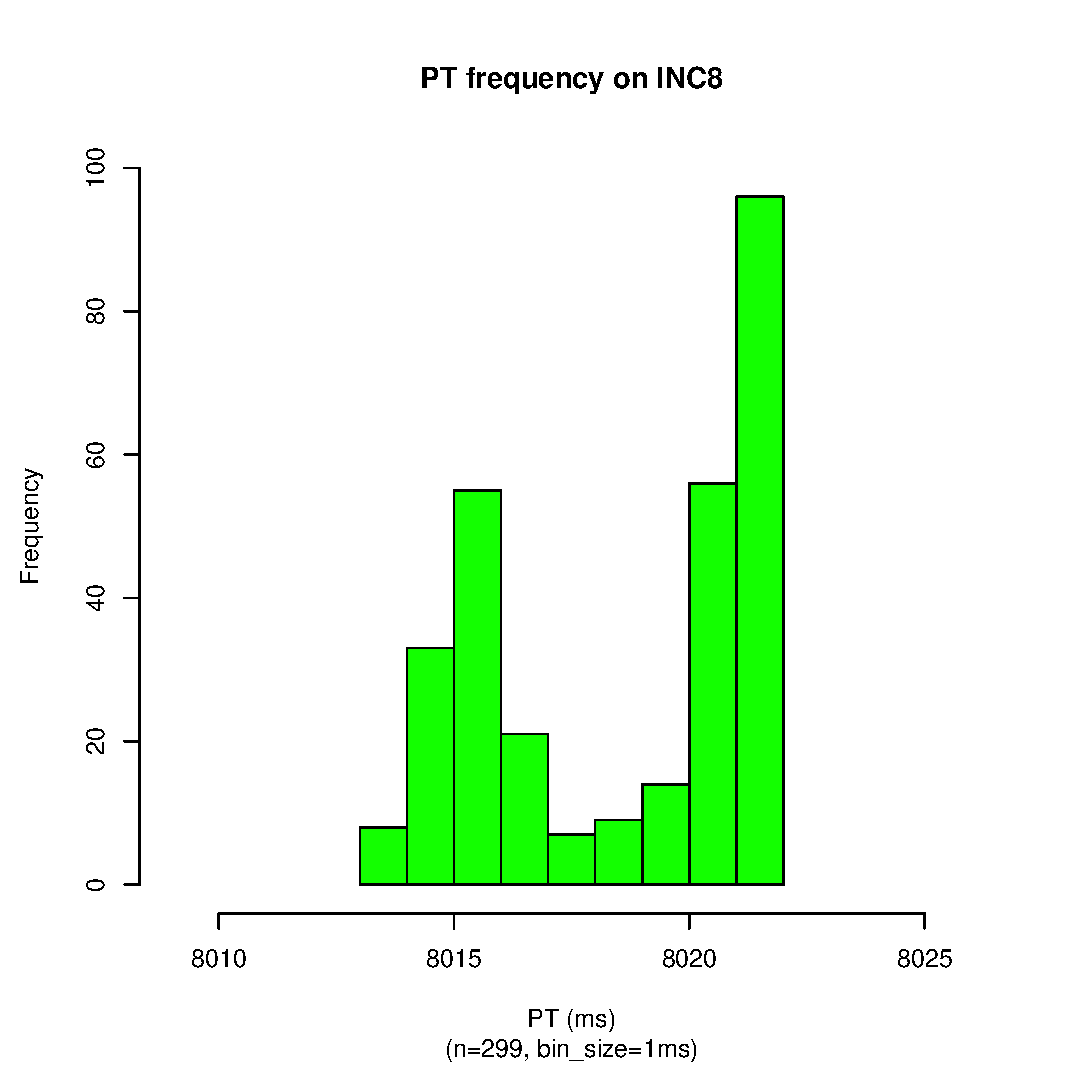
\includegraphics[scale=0.43]{sodb9/8_sec_pt_hist_v5.eps}
		\label{fig:inc8_hist_v5}
	}
	\caption{PT Histograms of INC1 ... INC8~\label{fig:s9_pt_hist1}}
\end{figure}

\begin{figure}[hp!]
	\centering
	\subfigure[PT frequency on INC16]{
		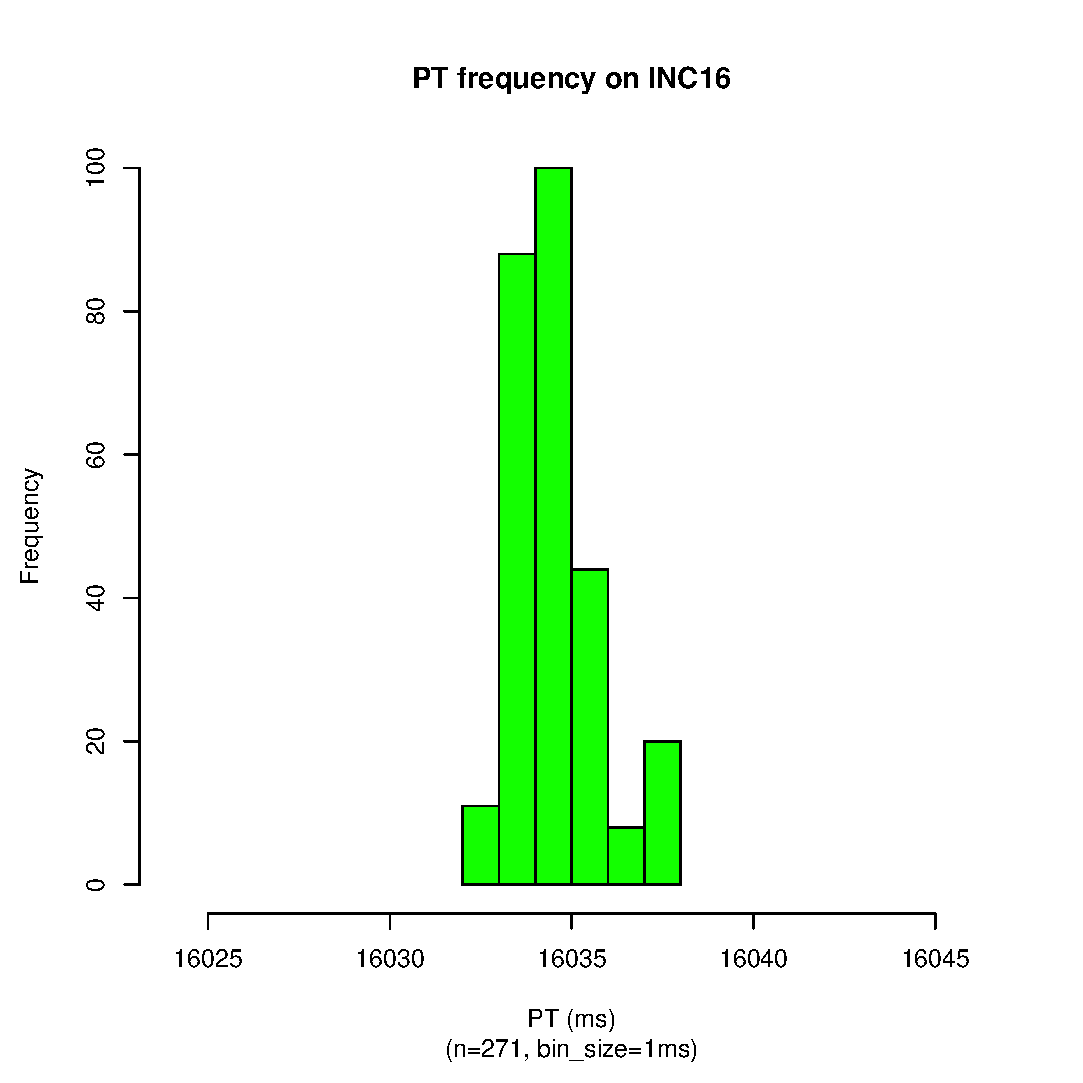
\includegraphics[scale=0.43]{sodb9/16_sec_pt_hist_v5.eps}
		\label{fig:inc16_hist_v5}
	}
	\subfigure[PT frequency on INC32]{
		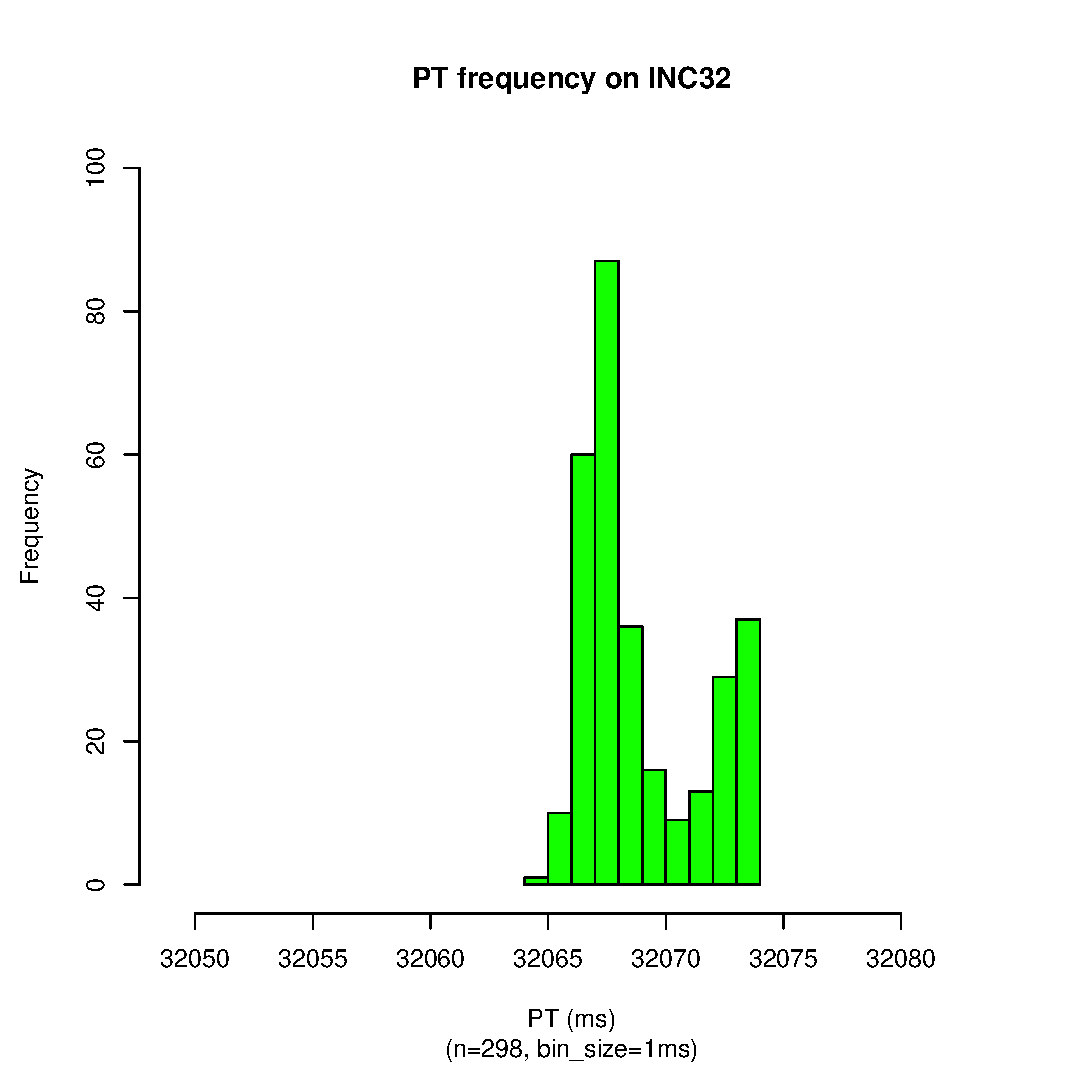
\includegraphics[scale=0.43]{sodb9/32_sec_pt_hist_v5.eps}
		\label{fig:inc32_hist_v5}
	}
	\subfigure[PT frequency on INC64]{
		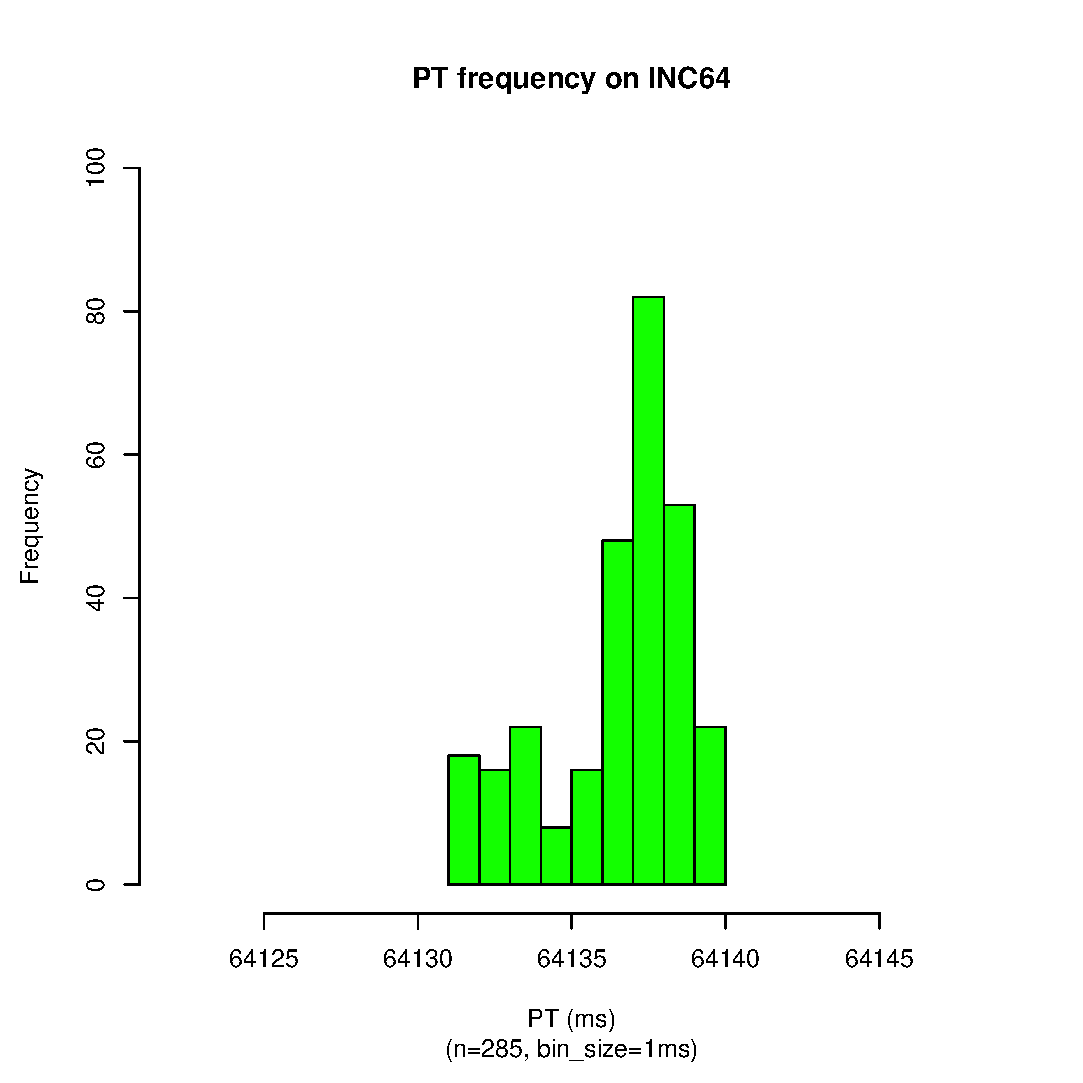
\includegraphics[scale=0.43]{sodb9/64_sec_pt_hist_v5.eps}
		\label{fig:inc64_hist_v5}
	}
	\caption{PT Histograms of INC16 ... INC64\label{fig:s9_pt_hist2}}
\end{figure}

\begin{figure}[hp!]
	\centering
	\subfigure[PT frequency on INC128]{
		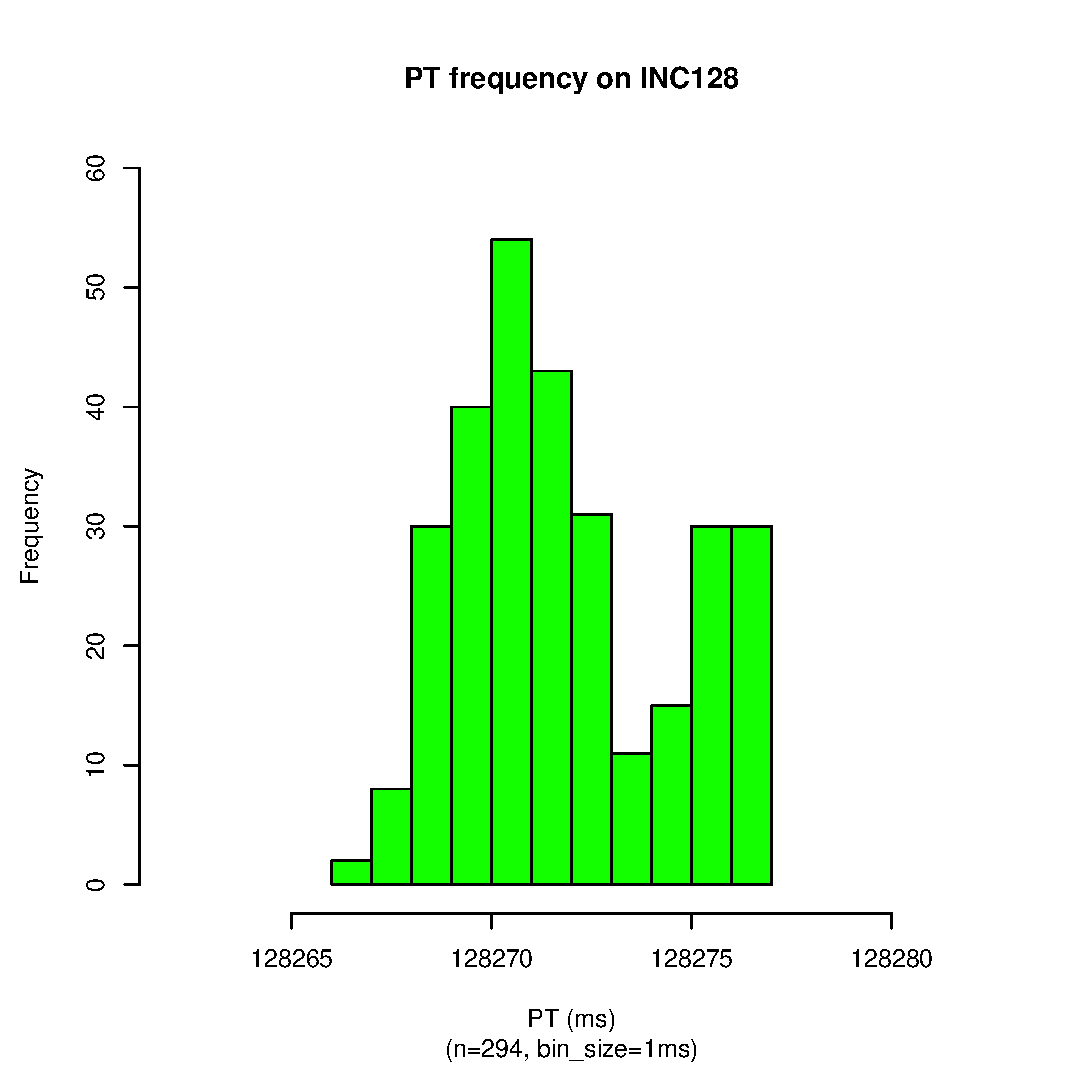
\includegraphics[scale=0.43]{sodb9/128_sec_pt_hist_v5.eps}
		\label{fig:inc128_hist_v5}
	}
	\subfigure[PT frequency on INC256]{
		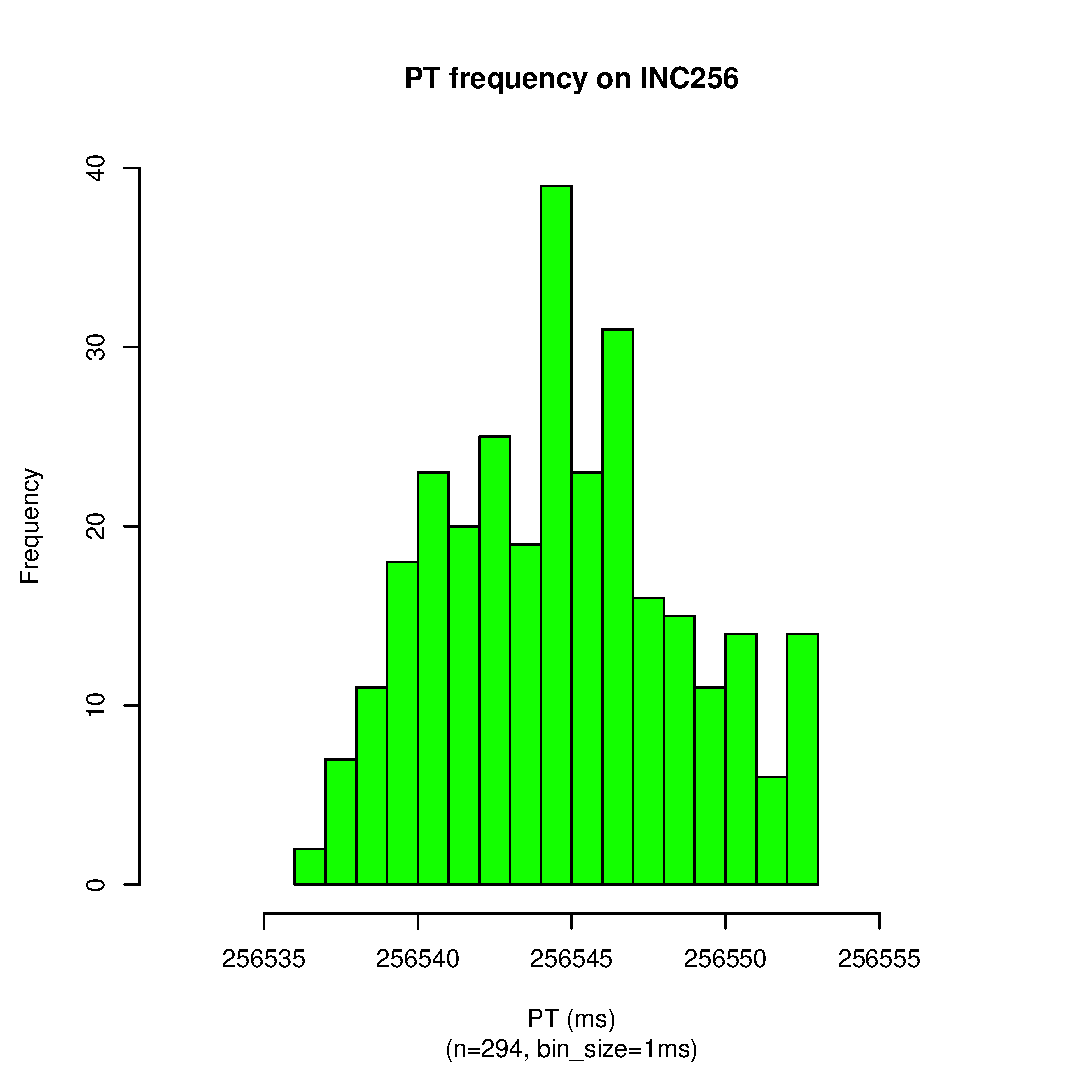
\includegraphics[scale=0.43]{sodb9/256_sec_pt_hist_v5.eps}
		\label{fig:inc256_hist_v5}
	}
	\subfigure[PT frequency on INC512]{
		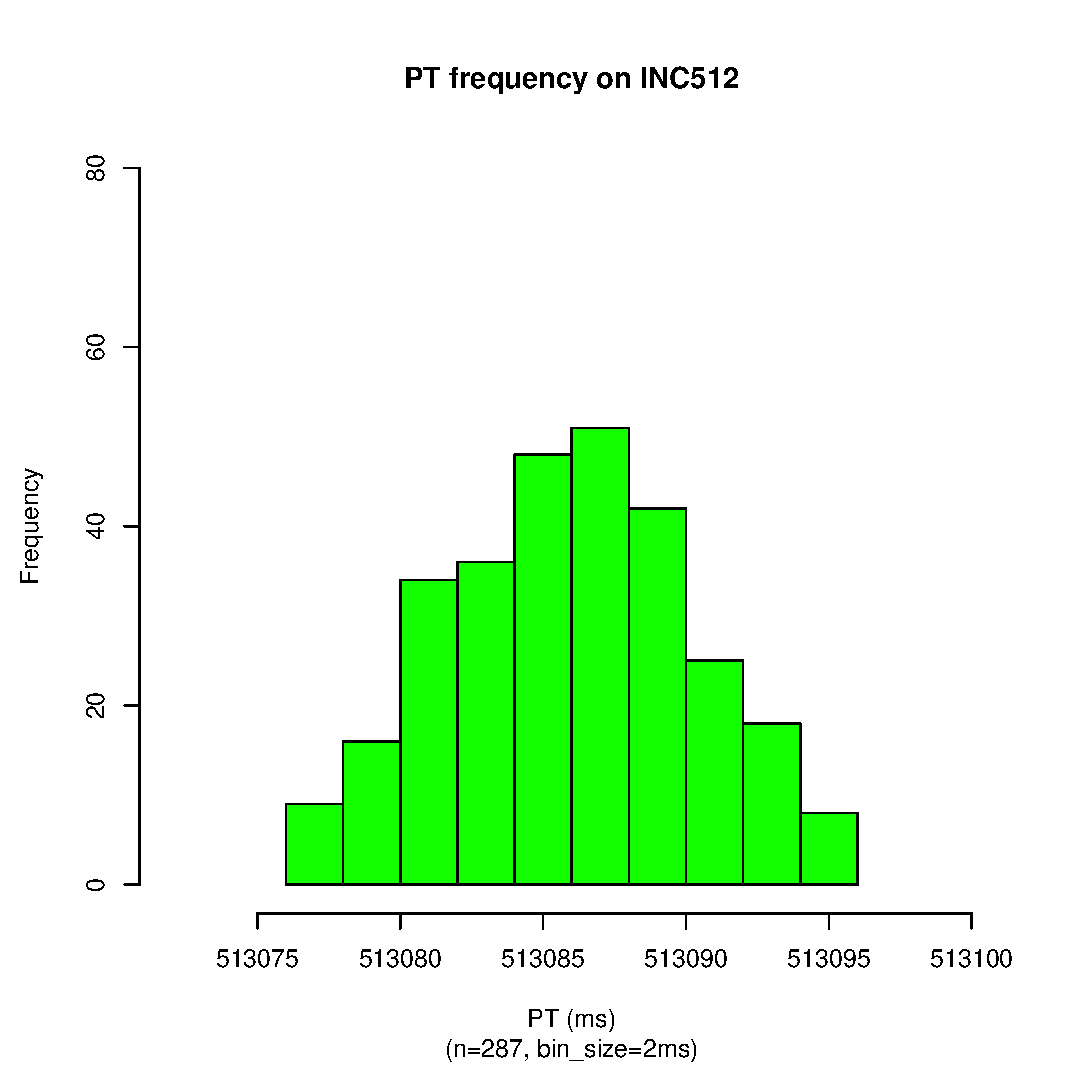
\includegraphics[scale=0.43]{sodb9/512_sec_pt_hist_v5.eps}
		\label{fig:inc512_hist_v5}
	}
	\subfigure[PT frequency on INC1024]{
		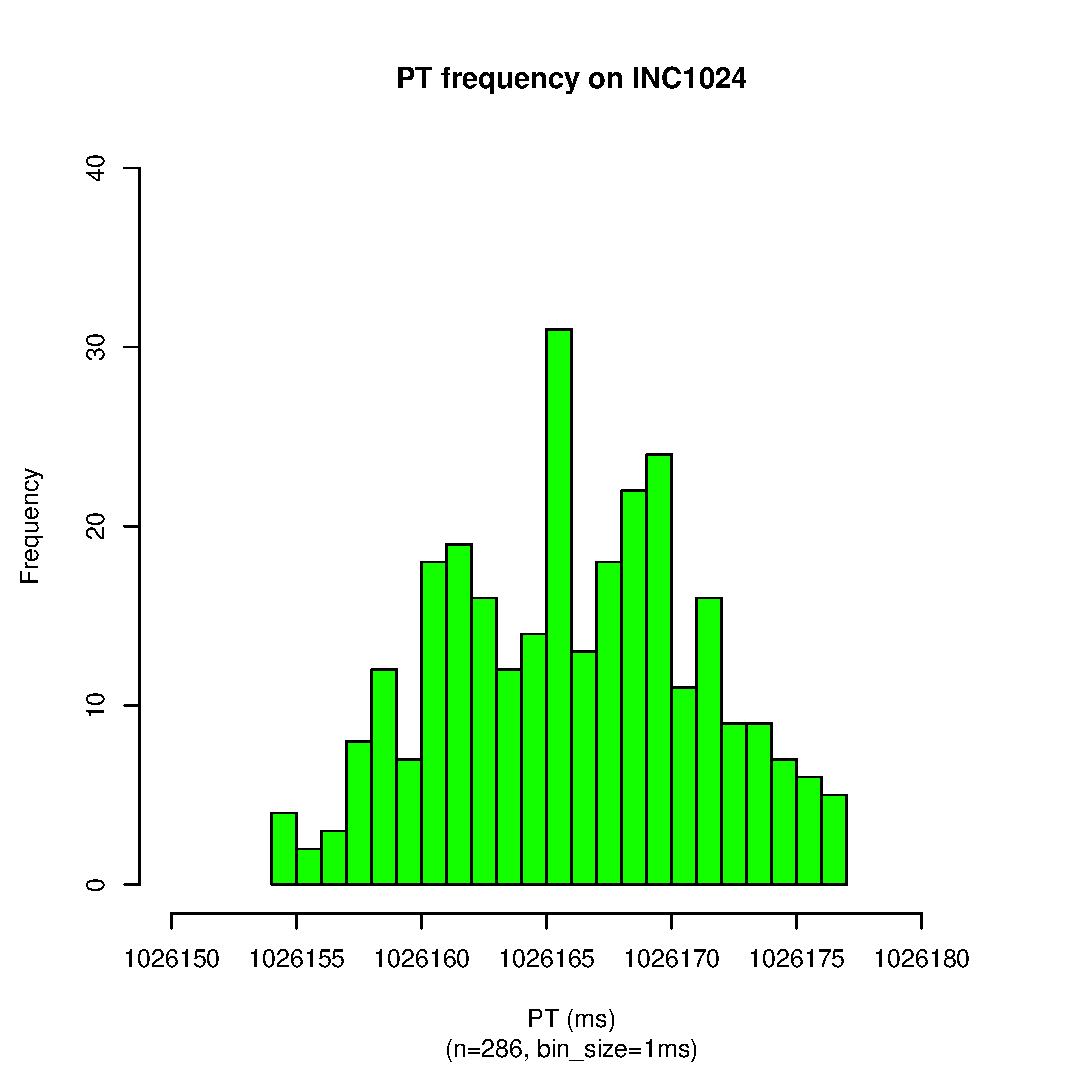
\includegraphics[scale=0.43]{sodb9/1024_sec_pt_hist_v5.eps}
		\label{fig:inc1024_hist_v5}
	}
	\caption{PT Histograms of INC256 ... INC1024~\label{fig:s9_pt_hist3}}
\end{figure}

\begin{figure}[hp!]
	\centering
	\subfigure[PT frequency on INC2048]{
		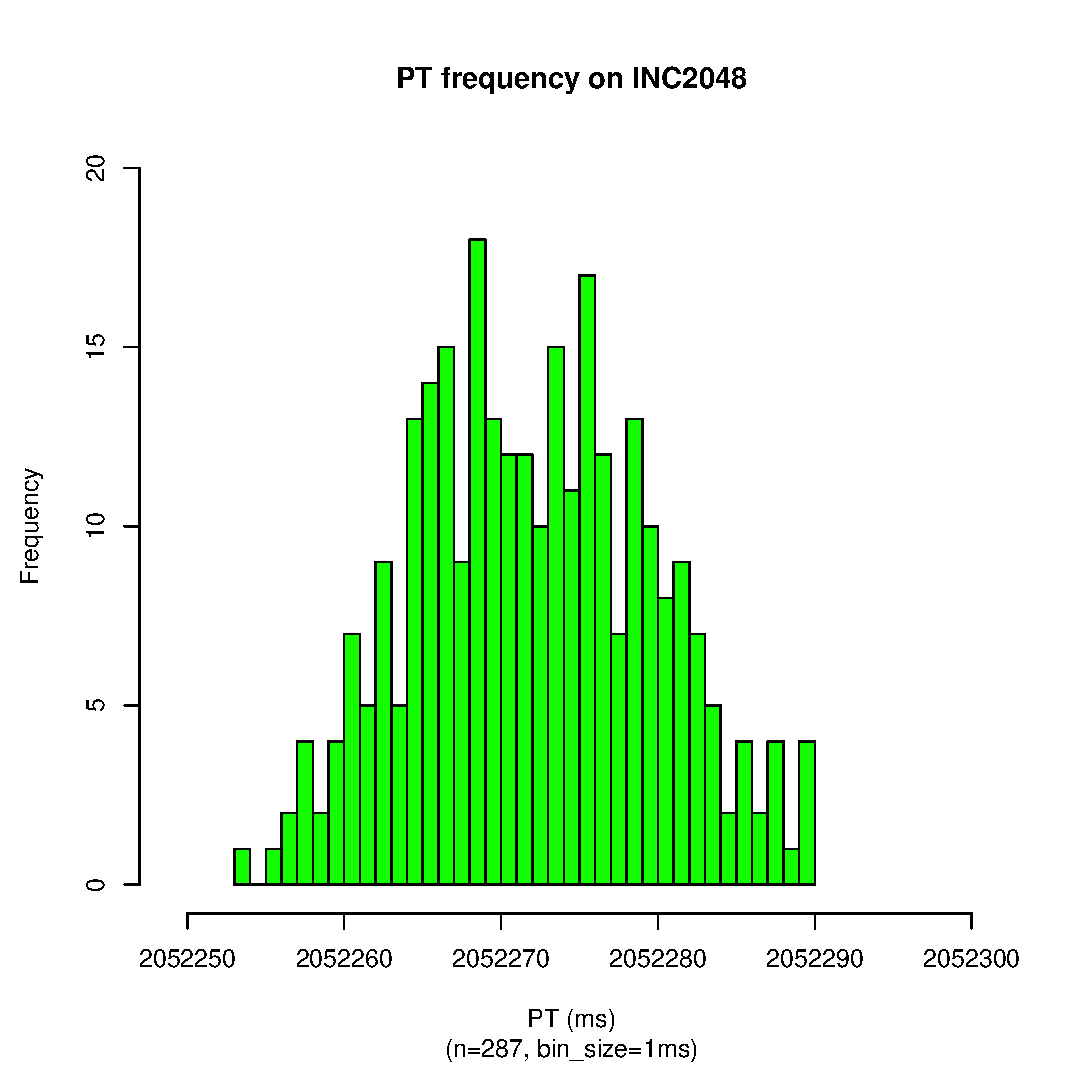
\includegraphics[scale=0.43]{sodb10/2048_sec_pt_hist_v5.eps}
		\label{fig:inc2048_hist_v5}
	}
	\subfigure[PT frequency on INC4096]{
		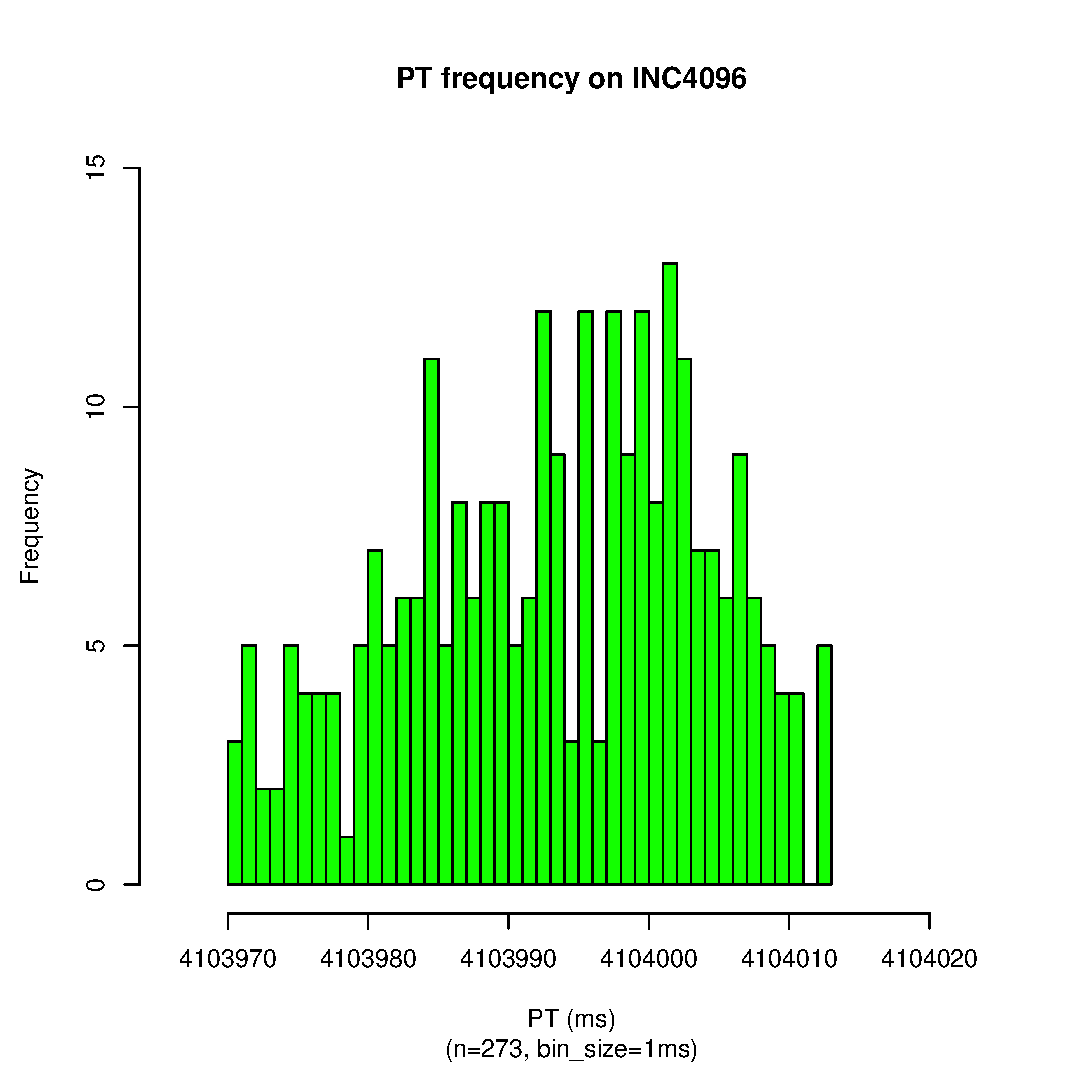
\includegraphics[scale=0.43]{sodb12/4096_sec_pt_hist_v5.eps}
		\label{fig:inc4096_hist_v5}
	}
	\subfigure[PT frequency on INC8192]{
		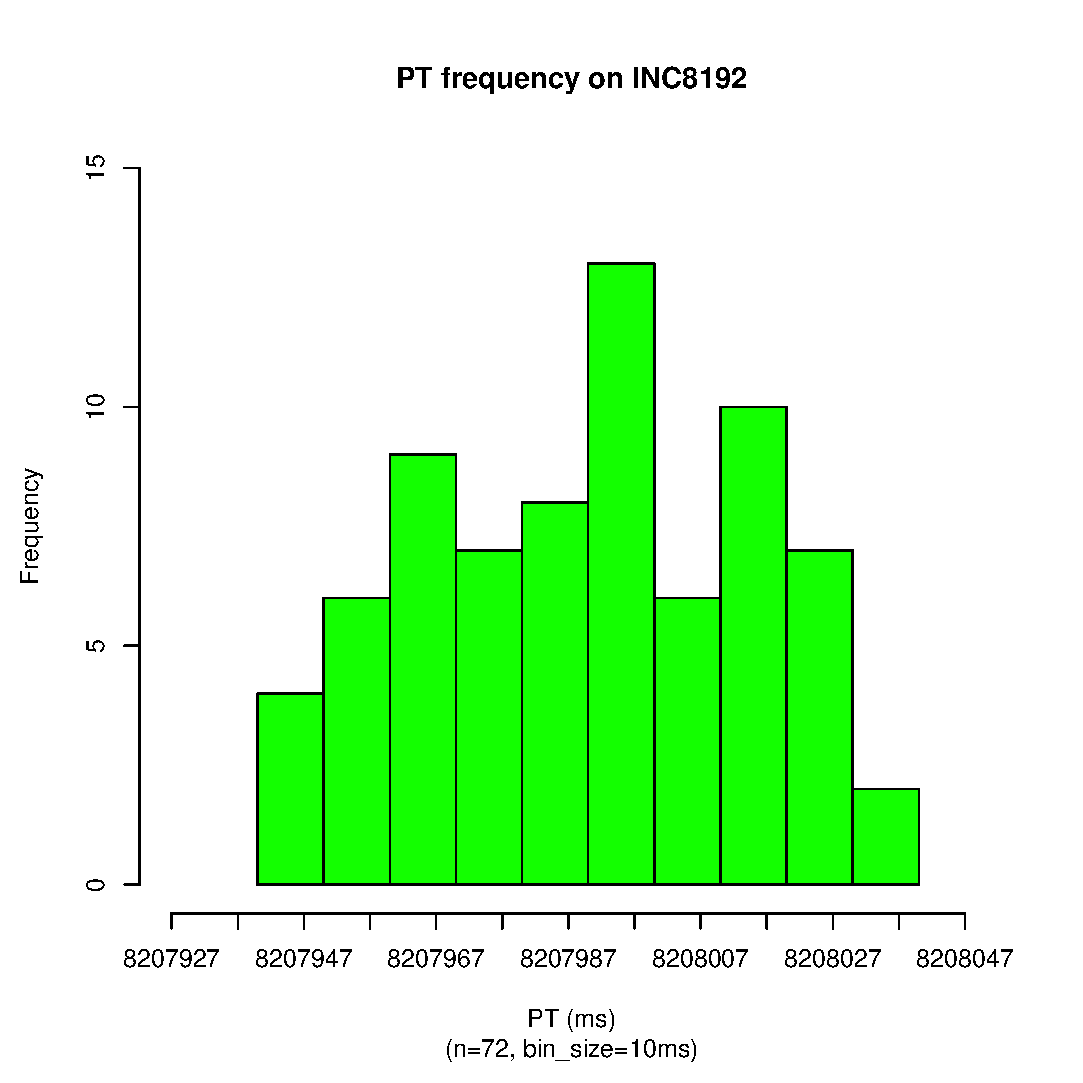
\includegraphics[scale=0.43]{sodb12/8192_sec_pt_hist2_v5.eps}
		\label{fig:inc8192_hist_v5}
	}
	\subfigure[PT frequency on INC16384]{
		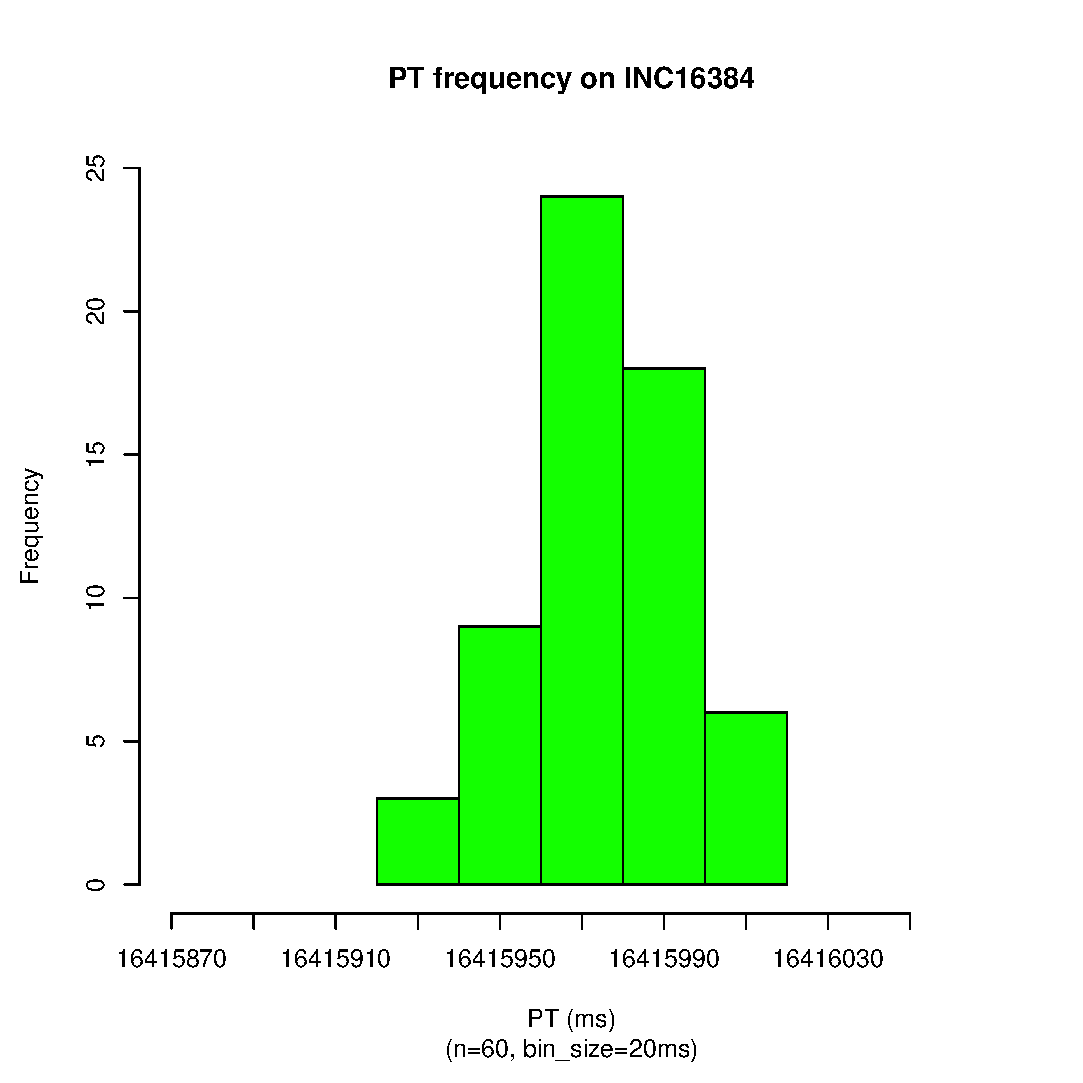
\includegraphics[scale=0.43]{sodb12/16384_sec_pt_hist2_v5.eps}
		\label{fig:inc16384_hist_v5}
	}
	\caption{PT Histograms of INC2048 and INC16384~\label{fig:s9_pt_hist4}}
\end{figure}

%\pagebreak
%
%\begin{figure}[hp!]
%	\centering
%	\subfigure[PT frequency on INC8192]{
%		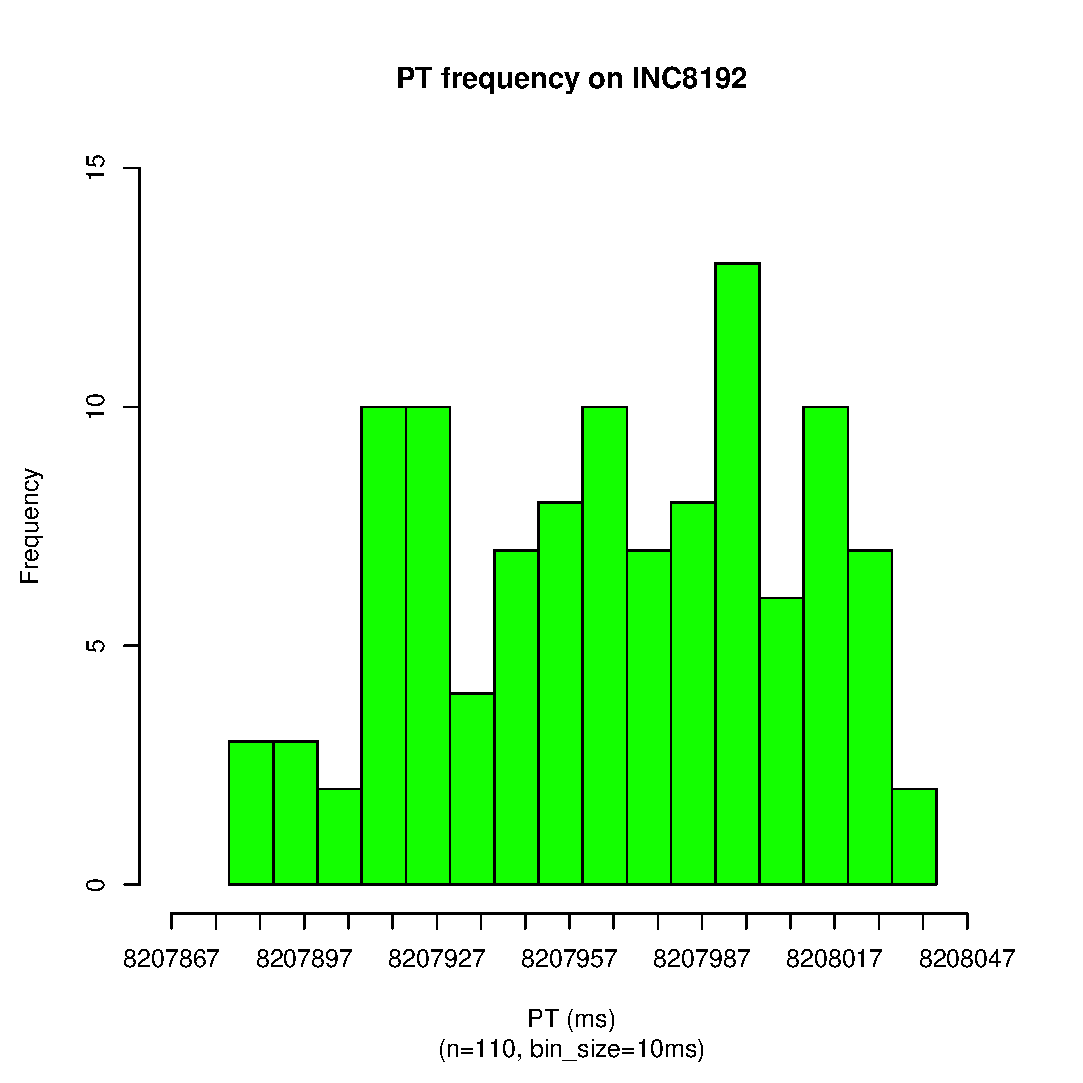
\includegraphics[scale=0.43]{sodb12/8192_sec_pt_hist_v5.eps}
%		\label{fig:inc8192_hist_all_v5}
%	}
%	\subfigure[PT frequency on INC16384]{
%		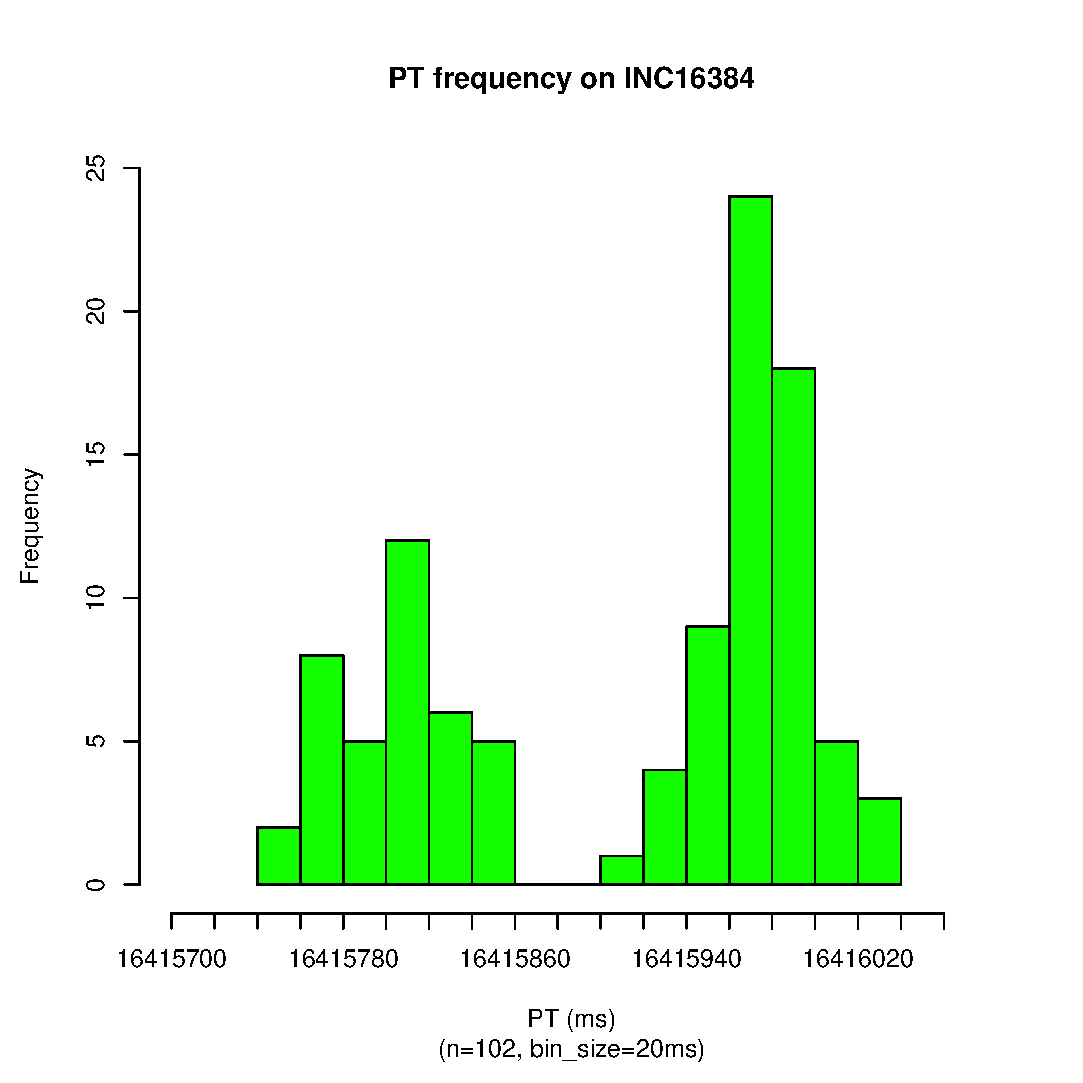
\includegraphics[scale=0.43]{sodb12/16384_sec_pt_hist_v5.eps}
%		\label{fig:inc16384_hist_all_v5}
%	}
%	\caption{PT Histograms of INC8192 and INC16384 [combined with 2015's run]~\label{fig:s9_pt_hist5}}
%\end{figure}
